% LaTeX support: latex@mdpi.com
% For support, please attach all files needed for compiling as well as the log file, and specify your operating system, LaTeX version, and LaTeX editor.

%=================================================================
\documentclass[algorithms,article,submit,pdftex,oneauthors]{Definitions/mdpi}

%--------------------
% Class Options:
%--------------------
%----------
% journal
%----------
% Choose between the following MDPI journals:
% acoustics, actuators, addictions, admsci, adolescents, aerobiology, aerospace, agriculture, agriengineering, agrochemicals, agronomy, ai, air, algorithms, allergies, alloys, analytica, analytics, anatomia, animals, antibiotics, antibodies, antioxidants, applbiosci, appliedchem, appliedmath, applmech, applmicrobiol, applnano, applsci, aquacj, architecture, arm, arthropoda, arts, asc, asi, astronomy, atmosphere, atoms, audiolres, automation, axioms, bacteria, batteries, bdcc, behavsci, beverages, biochem, bioengineering, biologics, biology, biomass, biomechanics, biomed, biomedicines, biomedinformatics, biomimetics, biomolecules, biophysica, biosensors, biotech, birds, bloods, blsf, brainsci, breath, buildings, businesses, cancers, carbon, cardiogenetics, catalysts, cells, ceramics, challenges, chemengineering, chemistry, chemosensors, chemproc, children, chips, cimb, civileng, cleantechnol, climate, clinpract, clockssleep, cmd, coasts, coatings, colloids, colorants, commodities, compounds, computation, computers, condensedmatter, conservation, constrmater, cosmetics, covid, crops, cryptography, crystals, csmf, ctn, curroncol, cyber, dairy, data, ddc, dentistry, dermato, dermatopathology, designs, devices, diabetology, diagnostics, dietetics, digital, disabilities, diseases, diversity, dna, drones, dynamics, earth, ebj, ecologies, econometrics, economies, education, ejihpe, electricity, electrochem, electronicmat, electronics, encyclopedia, endocrines, energies, eng, engproc, entomology, entropy, environments, environsciproc, epidemiologia, epigenomes, est, fermentation, fibers, fintech, fire, fishes, fluids, foods, forecasting, forensicsci, forests, foundations, fractalfract, fuels, future, futureinternet, futurepharmacol, futurephys, futuretransp, galaxies, games, gases, gastroent, gastrointestdisord, gels, genealogy, genes, geographies, geohazards, geomatics, geosciences, geotechnics, geriatrics, grasses, gucdd, hazardousmatters, healthcare, hearts, hemato, hematolrep, heritage, higheredu, highthroughput, histories, horticulturae, hospitals, humanities, humans, hydrobiology, hydrogen, hydrology, hygiene, idr, ijerph, ijfs, ijgi, ijms, ijns, ijpb, ijtm, ijtpp, ime, immuno, informatics, information, infrastructures, inorganics, insects, instruments, inventions, iot, j, jal, jcdd, jcm, jcp, jcs, jcto, jdb, jeta, jfb, jfmk, jimaging, jintelligence, jlpea, jmmp, jmp, jmse, jne, jnt, jof, joitmc, jor, journalmedia, jox, jpm, jrfm, jsan, jtaer, jvd, jzbg, kidneydial, kinasesphosphatases, knowledge, land, languages, laws, life, liquids, literature, livers, logics, logistics, lubricants, lymphatics, machines, macromol, magnetism, magnetochemistry, make, marinedrugs, materials, materproc, mathematics, mca, measurements, medicina, medicines, medsci, membranes, merits, metabolites, metals, meteorology, methane, metrology, micro, microarrays, microbiolres, micromachines, microorganisms, microplastics, minerals, mining, modelling, molbank, molecules, mps, msf, mti, muscles, nanoenergyadv, nanomanufacturing,\gdef\@continuouspages{yes}} nanomaterials, ncrna, ndt, network, neuroglia, neurolint, neurosci, nitrogen, notspecified, %%nri, nursrep, nutraceuticals, nutrients, obesities, oceans, ohbm, onco, %oncopathology, optics, oral, organics, organoids, osteology, oxygen, parasites, parasitologia, particles, pathogens, pathophysiology, pediatrrep, pharmaceuticals, pharmaceutics, pharmacoepidemiology,\gdef\@ISSN{2813-0618}\gdef\@continuous pharmacy, philosophies, photochem, photonics, phycology, physchem, physics, physiologia, plants, plasma, platforms, pollutants, polymers, polysaccharides, poultry, powders, preprints, proceedings, processes, prosthesis, proteomes, psf, psych, psychiatryint, psychoactives, publications, quantumrep, quaternary, qubs, radiation, reactions, receptors, recycling, regeneration, religions, remotesensing, reports, reprodmed, resources, rheumato, risks, robotics, ruminants, safety, sci, scipharm, sclerosis, seeds, sensors, separations, sexes, signals, sinusitis, skins, smartcities, sna, societies, socsci, software, soilsystems, solar, solids, spectroscj, sports, standards, stats, std, stresses, surfaces, surgeries, suschem, sustainability, symmetry, synbio, systems, targets, taxonomy, technologies, telecom, test, textiles, thalassrep, thermo, tomography, tourismhosp, toxics, toxins, transplantology, transportation, traumacare, traumas, tropicalmed, universe, urbansci, uro, vaccines, vehicles, venereology, vetsci, vibration, virtualworlds, viruses, vision, waste, water, wem, wevj, wind, women, world, youth, zoonoticdis
% For posting an early version of this manuscript as a preprint, you may use "preprints" as the journal. Changing "submit" to "accept" before posting will remove line numbers.

%---------
% article
%---------
% The default type of manuscript is "article", but can be replaced by:
% abstract, addendum, article, book, bookreview, briefreport, casereport, comment, commentary, communication, conferenceproceedings, correction, conferencereport, entry, expressionofconcern, extendedabstract, datadescriptor, editorial, essay, erratum, hypothesis, interestingimage, obituary, opinion, projectreport, reply, retraction, review, perspective, protocol, shortnote, studyprotocol, systematicreview, supfile, technicalnote, viewpoint, guidelines, registeredreport, tutorial
% supfile = supplementary materials

%----------
% submit
%----------
% The class option "submit" will be changed to "accept" by the Editorial Office when the paper is accepted. This will only make changes to the frontpage (e.g., the logo of the journal will get visible), the headings, and the copyright information. Also, line numbering will be removed. Journal info and pagination for accepted papers will also be assigned by the Editorial Office.

%------------------
% moreauthors
%------------------
% If there is only one author the class option oneauthor should be used. Otherwise use the class option moreauthors.

%---------
% pdftex
%---------
% The option pdftex is for use with pdfLaTeX. Remove "pdftex" for (1) compiling with LaTeX & dvi2pdf (if eps figures are used) or for (2) compiling with XeLaTeX.

%=================================================================
% MDPI internal commands - do not modify
\firstpage{1}
\makeatletter
\setcounter{page}{\@firstpage}
\makeatother
\pubvolume{1}
\issuenum{1}
\articlenumber{0}
\pubyear{2023}
\copyrightyear{2023}
%\externaleditor{Academic Editor: Firstname Lastname}
\datereceived{ }
\daterevised{ } % Comment out if no revised date
\dateaccepted{ }
\datepublished{ }
%\datecorrected{} % For corrected papers: "Corrected: XXX" date in the original paper.
%\dateretracted{} % For corrected papers: "Retracted: XXX" date in the original paper.
\hreflink{https://doi.org/} % If needed use \linebreak
%\doinum{}
%\pdfoutput=1 % Uncommented for upload to arXiv.org

%=================================================================
% Add packages and commands here. The following packages are loaded in our class file: fontenc, inputenc, calc, indentfirst, fancyhdr, graphicx, epstopdf, lastpage, ifthen, float, amsmath, amssymb, lineno, setspace, enumitem, mathpazo, booktabs, titlesec, etoolbox, tabto, xcolor, colortbl, soul, multirow, microtype, tikz, totcount, changepage, attrib, upgreek, array, tabularx, pbox, ragged2e, tocloft, marginnote, marginfix, enotez, amsthm, natbib, hyperref, cleveref, scrextend, url, geometry, newfloat, caption, draftwatermark, seqsplit
% cleveref: load \crefname definitions after \begin{document}

\usepackage{gensymb}
\usepackage{accents}
\usepackage{xspace}

%Definition des mises en page
\definecolor{gray75}{gray}{0.75}
\definecolor{gray95}{gray}{0.95}
\definecolor{gray50}{gray}{0.50}
\definecolor{gray40}{gray}{0.40}
\definecolor{redcolor}{rgb}{0.6,0.0,0.0}
\definecolor{greencolor}{rgb}{0.0,0.6,0.0}  % green color

% Definition des listings avec langage par défaut Python
\usepackage{listings}

\lstnewenvironment{FortranListing}[1][]
    {\lstset{language=[77]Fortran,#1}}{}

\lstnewenvironment{PythonListing}[1][]
    {\lstset{language=Python,morekeywords={as,assert,with,yield},#1}}{}


\lstset{language=Python,
keywordstyle=\color{redcolor},
numberstyle=\footnotesize\color{gray40},
numbers=left,
literate={-} {\textrm{-}}{1},
showstringspaces=false,
commentstyle=\color{gray50},
stringstyle=\color{greencolor},
basicstyle=\sffamily\small\upshape,
backgroundcolor=\color{gray95}
}

\usepackage[labelformat=simple]{subcaption}
\renewcommand\thesubfigure{\alph{subfigure}}
\DeclareCaptionLabelFormat{subcaptionlabel}{\normalfont(\textbf{#2}\normalfont)}
\captionsetup[subfigure]{labelformat=subcaptionlabel}

\DeclareRobustCommand{\w}{\mbox{\large\ensuremath{\mathsf{w}}}}
\DeclareRobustCommand{\dotp}{\boldsymbol{\cdot}}
\DeclareRobustCommand{\e}[1]{{\rm e}^{#1}}
\DeclareRobustCommand{\lay}[1]{_{[#1]}}
\DeclareRobustCommand{\Lay}[1]{\mbox{$[#1]$}}
\DeclareRobustCommand{\mdot}[1]{\accentset{\mbox{\bfseries .}}{#1}}
\DeclareRobustCommand{\ie}{i.e.,\@\xspace}
\DeclareRobustCommand{\eal}{et \emph{al.}\@\xspace}
\DeclareRobustCommand{\MSE}{\text{E}_\text{MS}}
\DeclareRobustCommand{\RMSE}{\text{E}_\text{RMS}}
\DeclareRobustCommand{\MARE}{\text{E}_\text{MAR}}
\DeclareRobustCommand{\ps}{\text{s}^{-1}}
\DeclareRobustCommand{\MPa}{\text{MPa}}
\DeclareRobustCommand{\GPa}{\text{GPa}}
\DeclareRobustCommand{\Sig}{\mbox{\large\ensuremath{\boldsymbol{\sigma}}}}
\DeclareRobustCommand{\Eps}{\mbox{\large\ensuremath{\boldsymbol{\varepsilon}}}}
\DeclareRobustCommand{\var}[1]{\textsf{#1}}

% This is used to add comments into the text
%
% Will have to be removed from final version
%
%\usepackage{soul}
%\usepackage{color}
%\definecolor{VWyellow}{RGB}{255,251,150}
%\DeclareRobustCommand{\OP}[1]{\begingroup\sethlcolor{VWyellow}\textcolor{red}{\hl{\textbf{O.P.:} #1}}\endgroup}
%\DeclareRobustCommand{\OPP}[1]{\begingroup\sethlcolor{VWyellow}\textcolor{red}{\hl{\textbf{O.P.:} In previous sentence #1}}\endgroup}

%=================================================================
% Please use the following mathematics environments: Theorem, Lemma, Corollary, Proposition, Characterization, Property, Problem, Example, ExamplesandDefinitions, Hypothesis, Remark, Definition, Notation, Assumption
%% For proofs, please use the proof environment (the amsthm package is loaded by the MDPI class).

%=================================================================
% Full title of the paper (Capitalized)
\Title{Comparing Activation Functions in Machine Learning for Finite Element Simulations in Thermomechanical Forming}

% MDPI internal command: Title for citation in the left column
\TitleCitation{Comparing Activation Functions in Machine Learning for Finite Element Simulations in Thermomechanical Forming}

% Author Orchid ID: enter ID or remove command
\newcommand{\orcidauthorA}{0000-0001-7367-5453} % Add \orcidA{} behind the author's name
%\newcommand{\orcidauthorB}{0000-0000-0000-000X} % Add \orcidB{} behind the author's name

% Authors, for the paper (add full first names)
\Author{Olivier Pantal\'{e}\orcidA{}}

%\longauthorlist{yes}

% MDPI internal command: Authors, for metadata in PDF
\AuthorNames{Olivier Pantal\'{e}}

% MDPI internal command: Authors, for citation in the left column
\AuthorCitation{Pantal\'{e}, O.}
% If this is a Chicago style journal: Lastname, Firstname, Firstname Lastname, and Firstname Lastname.

% Affiliations / Addresses (Add [XX] after \address if there is only one affiliation.)
\address[1]{Laboratoire Génie de Production, Institut National Polytechnique/Ecole Nationale d'Ingénieurs de Tarbes, Université de Toulouse, 47 Av d'Azereix, F-65016 Tarbes, France; Olivier.Pantale@enit.fr; Tel.: +33-562-442-933}

% Current address and/or shared authorship
%\firstnote{Current address: Affiliation 3.}
%\secondnote{These authors contributed equally to this work.}
% The commands \thirdnote{} till \eighthnote{} are available for further notes

%\simplesumm{} % Simple summary

%\conference{} % An extended version of a conference paper

% Abstract (Do not insert blank lines, i.e. \\)
\abstract{Finite element (FE) simulations have been effective in simulating thermomechanical forming processes, yet challenges arise when applying them to new materials due to nonlinear behaviors.
To address this, machine learning techniques and artificial neural networks play an increasingly vital role in developing complex models.
This paper presents an innovative approach to parameter identification in flow laws, utilizing an artificial neural network that learns directly from test data and automatically generates a Fortran subroutine for the Abaqus standard or explicit FE codes.
We investigate the impact of activation functions on prediction and computational efficiency by comparing Sigmoid, Tanh, ReLU, Swish, Softplus, and the less common Exponential function.
Despite its infrequent use, the Exponential function demonstrates noteworthy performance and reduced computation times.
Model validation involves comparing predictive capabilities with experimental data from compression tests, and numerical simulations confirm the numerical implementation in the Abaqus explicit FE code.}

% Keywords
\keyword{Constitutive Behavior; ANN Flow Law; Numerical Implementation; User Hardening; Activation Functions; Abaqus}

% The fields PACS, MSC, and JEL may be left empty or commented out if not applicable
%\PACS{J0101}
%\MSC{}
%\JEL{}

%%%%%%%%%%%%%%%%%%%%%%%%%%%%%%%%%%%%%%%%%%
% Only for the journal Diversity
%\LSID{\url{http://}}

%%%%%%%%%%%%%%%%%%%%%%%%%%%%%%%%%%%%%%%%%%
% Only for the journal Applied Sciences
%\featuredapplication{Authors are encouraged to provide a concise description of the specific application or a potential application of the work. This section is not mandatory.}
%%%%%%%%%%%%%%%%%%%%%%%%%%%%%%%%%%%%%%%%%%

%%%%%%%%%%%%%%%%%%%%%%%%%%%%%%%%%%%%%%%%%%
% Only for the journal Data
%\dataset{DOI number or link to the deposited data set if the data set is published separately. If the data set shall be published as a supplement to this paper, this field will be filled by the journal editors. In this case, please submit the data set as a supplement.}
%\datasetlicense{License under which the data set is made available (CC0, CC-BY, CC-BY-SA, CC-BY-NC, etc.)}

%%%%%%%%%%%%%%%%%%%%%%%%%%%%%%%%%%%%%%%%%%
% Only for the journal Toxins
%\keycontribution{The breakthroughs or highlights of the manuscript. Authors can write one or two sentences to describe the most important part of the paper.}

%%%%%%%%%%%%%%%%%%%%%%%%%%%%%%%%%%%%%%%%%%
% Only for the journal Encyclopedia
%\encyclopediadef{For entry manuscripts only: please provide a brief overview of the entry title instead of an abstract.}

%%%%%%%%%%%%%%%%%%%%%%%%%%%%%%%%%%%%%%%%%%
% Only for the journal Advances in Respiratory Medicine
%\addhighlights{yes}
%\renewcommand{\addhighlights}{%

%\noindent This is an obligatory section in “Advances in Respiratory Medicine”, whose goal is to increase the discoverability and readability of the article via search engines and other scholars. Highlights should not be a copy of the abstract, but a simple text allowing the reader to quickly and simplified find out what the article is about and what can be cited from it. Each of these parts should be devoted up to 2~bullet points.\vspace{3pt}\\
%\textbf{What are the main findings?}
% \begin{itemize}[labelsep=2.5mm,topsep=-3pt]
% \item First bullet.
% \item Second bullet.
% \end{itemize}\vspace{3pt}
%\textbf{What is the implication of the main finding?}
% \begin{itemize}[labelsep=2.5mm,topsep=-3pt]
% \item First bullet.
% \item Second bullet.
% \end{itemize}
%}

%%%%%%%%%%%%%%%%%%%%%%%%%%%%%%%%%%%%%%%%%%
\begin{document}

%----------------------------------------------------------------------------------
\section{Introduction}\label{sec:Introduction}
%----------------------------------------------------------------------------------

In industry and research, numerical simulations are commonly employed to predict the behavior of structures under severe thermomechanical conditions, such as high-temperature forming of metallic materials.
These simulations rely on finite element (FE) codes, like Abaqus~\cite{Abaqus}, or academic codes.
The accuracy of these simulations is heavily influenced by constitutive equations and the identification of their parameters through experimental tests.
These tests, conducted under conditions similar to the actual service loading, involve quasi-static or dynamic tensile/compression tests, thermomechanical simulators (e.g., Gleeble~\cite{Lin-2009-MFS, Bennett-2010-C, Kumar-2016-TMS, Yu-2019-RCR}), or impact tests using gas guns or Hopkinson bars~\cite{Kolsky-1949-IMP}.
The choice and formulation of behavior laws and the accurate identification of coefficients from experiments are crucial for obtaining reliable simulation results.

%----------------------------------------------------------------------------------
\subsection{Constitutive behavior and material flow law}\label{subsec:ConstBehavior}
%----------------------------------------------------------------------------------

Thermomechanical behavior laws used in numerical integration algorithms such as the radial-return method~\cite{Ponthot-2002-USU} involve nonlinear flow law functions due to the complex nature of materials and associated phenomena like work hardening, dislocation movement, structural hardening, and phase transformations.
The applicability of these flow laws is confined to specific ranges of deformations, strain rates, and temperatures.
In the context of simulating forming processes, these behavior laws dictate how the material's flow stress~$\sigma$ depends on three key input variables: strain~$\varepsilon$, strain rate~$\mdot{\varepsilon}$, and temperature~$T$.
The general form of the flow law is expressed through a mathematical equation:
\begin{equation}
\sigma = \Sig\left(\varepsilon, \mdot{\varepsilon}, T\right).\label{eq:GenFlow}
\end{equation}

The historical development of behavior laws for simulating hot forming processes, beginning in the 1950s, involved the use of power laws to describe strain/stress relationships, later adapted to incorporate temperature effects.
In the 1970s, thermomechanical models evolved to include time dependence, linking flow laws to strain rate and time.
Notable models like the Johnson--Cook~\cite{Johnson-1983-CMD}, Zerilli--Armstrong~\cite{Zerilli-1987-DMB}, and Arrhenius~\cite{Jonas-1969} flow laws emerged and are commonly used in forming process simulations.
The selection of a flow law for simulating material behavior in finite element analysis is crucial, and it should be based on experimental tests conducted under conditions resembling real-world applications.
Researchers face a challenge in choosing the appropriate flow law after characterizing experimental behavior.
This decision is influenced by the availability of flow laws within the finite element analysis software being used.
For instance, users of Abaqus FE code~\cite{Abaqus} may prefer the native implementation of the Johnson--Cook flow law.
Opting for alternative flow laws like Zerilli--Armstrong or Arrhenius requires users to personally compute material yield stress~$\sigma$ through a VUMAT subroutine in Fortran, which is time-consuming, demands expertise in flow law formulations, numerical integration, Fortran programming, and model development and testing~\cite{Gao-2007-FRT, Ming-2018-ERV, Liang-2022}.

Developing and implementing a user behavior law on the Abaqus code involves calculating~$\sigma$, defined by Equation~(\ref{eq:GenFlow}), and its three derivatives with respect to $\varepsilon$, $\mdot{\varepsilon}$, and $T$.
This process becomes complex and time-consuming with increasing flow law complexity.
The choice of a flow law for simulating thermomechanical forming is influenced by both material behavior and process physics, but primarily by the flow laws available in the FE code.
The decision often prioritizes the availability of a flow law over the quality of the model, making the choice of flow law a critical factor in the simulation process.
In Tize Mha \eal~\cite{Tize-2023-IEP}, several flow laws were investigated through experimental compression tests on a Gleeble-3800 thermomechanical simulator for P20 medium-carbon steel used in foundry mold production.
The examined flow laws included Johnson--Cook, Modified Zerilli--Armstrong, Arrhenius, Hensel--Spittle, and PTM.
The findings revealed that, among the tested strain rates and temperatures, only the Arrhenius flow law accurately replicated the compression behavior of the material with a fidelity suitable for industrial applications.

Based on all these considerations, we have presented a novel approach, as outlined in Pantalé \eal~\cite{Pantale-2021-EIN, Pantale-2023-DIA}, for formulating flow laws.
This approach leverages the capacity of artificial neural networks (ANNs) to act as universal approximators, a concept established by Minsky \eal~\cite{Minsky-1969-PIC} and Hornik \eal~\cite{Hornik-1989-MFN}.
With this innovative method, there is no longer a prerequisite to predefine a mathematical form for the constitutive equation before its use in a finite element simulation.

Artificial neural networks have been investigated in the field of thermomechanical plasticity modeling as reported by Gorji \eal~\cite{Gorji-2020} or Jamli \eal~\cite{Jamli-2019-SNN}.
These studies explore the application of ANNs in FE investigation of metal forming processes and their characterization of meta-materials.
Lin \eal~\cite{Lin-2008} successfully applied an ANN to predict the yield stress of 42CrMo4 steel in hot compression, and ANNs have demonstrated success in predicting the flow stress behavior under hot working conditions~\cite{Stoffel-2018-ANN, Stoffel-2019-NNB}.
They have also been applied recently in micromechanics for polycrystalline metals by Ali \eal~\cite{Ali-2019-AAN}.
The domain of application has been extended to dynamic recrystallization of metal alloys by Wang \eal~\cite{Wang-2021-ANN}.
Some approaches mix analytical and ANN flow laws such as for example the work proposed by Cheng \eal~\cite{Cheng-2022-CWD} where the authors use a combination of an ANN with the Arrhenius equation to model the behavior of a GH4169 superalloy.
ANN behavior laws can also include chemical composition of materials in their formulation to increase the performance during simulation hot deformation for high-Mn steels with different concentrations as proposed by Churyumov \eal~\cite{Churyumov-2023-PTS}.

In the majority of the works presented in the previous paragraph, the authors work either on the proposal of a neural network model and its identification in relation to experimental tests, or on the use of ANNs within the framework of a numerical simulation of a process.
The approach proposed here is more complete in that we identify a neural network from experimental tests (in our case, cylinder compression tests performed on a Gleeble device), then identify the network parameters.
We then implement this ANN in Abaqus as a user subroutine in Fortran, and subsequently validate and use this network in numerical simulations.
This can be done for either Abaqus explicit or Abaqus standard since we can generate the Fortran subroutines for both versions of the code.
We therefore work on the entire calculation chain, from experimental data acquisition, through network formulation and learning, to implementation and use.

In this study, we will focus only on the use of the explicit version of Abaqus, since the computation of the flow stress in an explicit integration scheme becomes very CPU intensive due to the integration method, and variations in the performance of this implementation have a significant impact on the total CPU time.
On the other hand, in an implicit integration scheme, as used in the Abaqus standard, most of the time is spent in inverting the linear system of equations, therefore variations in the performance of the stress computation has no influence on the final result, hoping that the stress is calculated correctly.

%----------------------------------------------------------------------------------
\subsection{Experimental tests and data}\label{subsec:ExpTests}
%----------------------------------------------------------------------------------

This study uses a medium-carbon steel, type P20, with the chemical composition presented in Table~\ref{tab:Composition}.
\begin{table}[H]
\caption{Chemical composition of medium-carbon steel. Fe = balance.}
\newcolumntype{L}{>{\raggedright\arraybackslash}X}
\newcolumntype{C}{>{\centering\arraybackslash}X}
\begin{tabularx}{\textwidth}{lCCCCCCC}
\toprule
\textbf{Element} & \textbf{C} & \textbf{Mn} & \textbf{Mo} & \textbf{Si} & \textbf{Ni} & \textbf{Cr} & \textbf{Cu} \\
\midrule
Wt~\% %MDPI: Not necessary
 & $0.30$ & $0.89$ & $0.52$ & $0.34$ & $0.68$ & $1.86$ & $0.17$ \\
\bottomrule
\end{tabularx}
\label{tab:Composition}
\end{table}

The experiments used in this study mirror those previously conducted by Tize Mha \eal~\cite{Tize-2023-IEP}.
These tests involve hot compression on a Gleeble-3800 of P20 steel cylinders with initial dimensions of ~$\phi_{0}=10$~mm and~$h_{0}=15$~mm.
Only the most relevant information about those experiments is reported here after.
In order to have a more complete knowledge about the compression tests conducted during this study, we refer to Tize Mha \eal~\cite{Tize-2023-IEP}.
%The imposed displacement was set to~$d=7.5$~mm, resulting in a reduction of~$50\%$ of the initial height.
Hot compression tests were performed for five temperatures, $[1050,1100,1150,1200,1250]~\celsius$ and six strain rates $[0.001,0.01,0.1,1,2,5]~\ps$.
Figure~\ref{fig:RawData} reports a plot of all 30 strain/stress curves extracted from the experiments.
\begin{figure}[h!]
\centering
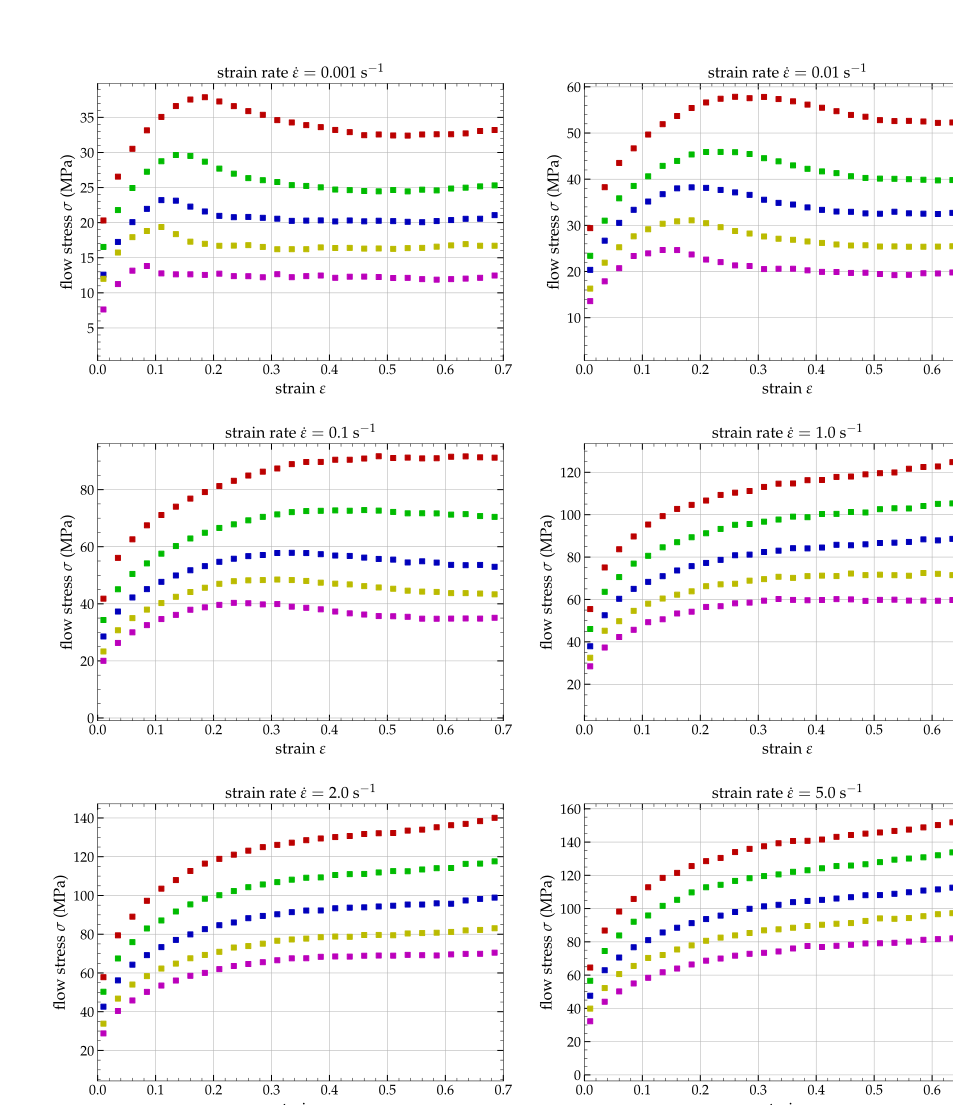
\includegraphics[width=0.9\columnwidth]{Figures/3Cr2Mo-raw}
\caption{Stress/strain curves of P20 alloy extracted from the Gleeble device for the five temperatures ($T$) and six strain rates ($\mdot{\varepsilon}$).}
\label{fig:RawData}
\end{figure}
The experimental database is composed of all strain/stress data for all 30 couples of strain rate and temperature.
Each strain/stress curve contains 701 equidistant strains $\varepsilon=[0.0,0.7]$ in~$\Delta\varepsilon=0.001$ increments.
The complete database contains~$21~030$ quadruplets ($\varepsilon$, $\mdot{\varepsilon}$, $T$ and~$\sigma$).
This dataset will be used here after to identify the ANN flow law parameters depending on the selected hyperparameters of the ANNs.

Section~\ref{sec:ANN} is dedicated to the presentation of the ANN based flow law.
The first part is dedicated to a reminder of the basic notions on ANNs, with a section on the choice of activation functions to be used in the formulation.
The architecture chosen for the formulation of the flow laws based on a two-hidden-layer network will then be presented, together with the formulation of the derivatives of the output with regard to the input variables.
The learning methodology and the results in terms of network performance as a function of the activation functions selected will then be presented.
Section~\ref{sec:Numerical} is dedicated to the FE simulation of a compression test using the explicit version of Abaqus, integrating the ANN implemented as a user routine in Fortran.
The quality of the numerical solution obtained and its performance in terms of computational cost will be analyzed as a function of the network structure.
Finally, the last section concerns conclusions and recommendations.

%----------------------------------------------------------------------------------
\section{Artificial Neural Network flow law}\label{sec:ANN}
%----------------------------------------------------------------------------------

As previously proposed by Pantalé \eal~\cite{Pantale-2021-EIN, Pantale-2023-DIA}, the employed methodology involves embedding the flow law, defined by a trained ANN, into the Abaqus code as a Fortran subroutine.
The ANN is trained using the experiments, as introduced in Section~\ref{sec:Introduction}, to compute the flow stress~$\sigma$ as a function of~$\varepsilon$, $\mdot{\varepsilon}$ and $T$.
Following the training phase, the ANN's weights and biases are transcribed into a Fortran subroutine, which is then compiled and linked with Abaqus libraries.
This integration enables Abaqus to incorporate the thermomechanical behavior by computing the flow stress and its derivatives ($\partial\sigma/\partial\varepsilon$, $\partial\sigma/\partial\mdot{\varepsilon}$, and $\partial\sigma/\partial T$) essential for the radial-return algorithm within the FE code.

%----------------------------------------------------------------------------------
\subsection{Artificial Neural Network equations}\label{subsec:ANN-eqn}
%----------------------------------------------------------------------------------

%----------------------------------------------------------------------------------
\subsubsection{Network architecture}\label{subsubsec:ANN-arch}
%----------------------------------------------------------------------------------

As illustrated in Figure~\ref{fig:ANN-2HL}, the ANN used for computing $\sigma$ from $\varepsilon$, $\mdot{\varepsilon}$ and $T$ is a two hidden layers network.
\begin{figure}[h!]
\centering
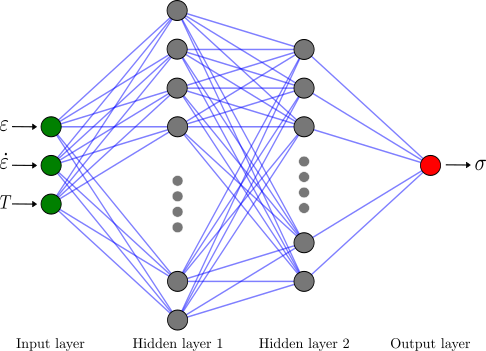
\includegraphics[width=0.55\columnwidth]{Figures/ANN-2HL}
\caption{Two hidden layers ANN architecture with 3 inputs ($\varepsilon$, $\mdot{\varepsilon}$ and~$T$) and 1 output ($\sigma$).}
\label{fig:ANN-2HL}
\end{figure}
The input of the neural network is a three component vector noted~$\overrightarrow{x}$.
Layer~\Lay{k}, composed of~$n$ neurons, computes the weighted sum of the outputs~$\overrightarrow{\hat{y}}\lay{k-1}$ of previous layer~\Lay{k-1}, composed of~$m$ neurons, according the equation:
\begin{equation}
\overrightarrow{y}\lay{k} = \w\lay{k} \cdot \overrightarrow{\hat{y}}\lay{k-1}+ \overrightarrow{b}\lay{k}\label{eq:ANN-y},
\end{equation}
where~$\overrightarrow{y}\lay{k}$ are the internal values of the neurons resulting the summation at the layer level~\Lay{k}, $\w\lay{k}$ is the weights matrix~$[n\times m]$ linking layer~\Lay{k} and layer~\Lay{k-1}, $\overrightarrow{b}\lay{k}$ is the bias vector of layer~\Lay{k} and~$\overrightarrow{\hat{y}}\lay{k-1}$ is the output vector of layer~\Lay{k-1} result of the activation function defined here-after.

The number of learning parameters~$N$ for any layer~\Lay{k} is the sum of the weights and biases in that layer, expressed as~$N=n(m+1)$.
Following the summation operation outlined in Equation (\ref{eq:ANN-y}), each hidden layer ~\Lay{k} produces an output vector~$\overrightarrow{\hat{y}}\lay{k}$ computed through an activation function~$f\lay{k}$, as defined by the subsequent equation:
\begin{equation}
\overrightarrow{\hat{y}}\lay{k}=f\lay{k}(\overrightarrow{y}\lay{k}).
\label{eq:ANN-f}
\end{equation}
This process is repeated for each hidden layer of the ANN until we reach the output layer where the formulation differ, so that the output~$s$ of the neural network is given by:
\begin{equation}
s = \overrightarrow{w}^T \dotp \overrightarrow{\hat{y}}\lay{2} + b\label{eq:ANN-s},
\end{equation}
where~$\overrightarrow{w}$ is the vector of the output weights of the ANN and~$b$ is the bias associated to the output neuron.
As usually done in a regression approach, there is no activation function associated to the output neuron of the network (or some authors consider here a linear activation function).

%----------------------------------------------------------------------------------
\subsubsection{Activation functions}\label{subsubsec:ANN-act}
%----------------------------------------------------------------------------------

At the heart of ANNs lies the concept of activation functions, pivotal elements that determine how information is transformed within the neurons.
Choosing activation functions is a critical design decision, as these functions greatly influence the network's capacity to learn and represent complex patterns in data.
The selection of activation functions is guided by their distinct properties, including non-linearity, differentiability, and computational efficiency.

In regression ANNs, the choice of activation functions is typically driven by the need to approximate continuous output values rather than class labels.
Many studies have been proposed concerning the right activation function to use depending on the physical problem to solve such as the review proposed by Dubey \eal~\cite{Dubey-2022-AFD} or Jagtap \eal~\cite{Jagtap-2023-HIA}.
The activation function is essential for introducing non-linearity into a neural network, allowing it to capture non-linear features.
Without this non-linearity, the network would behave like a linear regression model, as emphasized by Hornik \eal~\cite{Hornik-1989-MFN}.
A number of activations functions can be used in neural networks.

In our previous published work~\cite{Pantale-2021-EIN, Pantale-2023-DIA}, we have mostly used the Sigmoid activation function for the ANN flow laws.
In the present paper, we are going to explore other activations functions and their influence on the final results, up-to the implementation into a FE software.
Among the number of activations functions available in the literature, we have selected the six ones reported in Figure~\ref{fig:ActFunctions}.
\begin{figure}[h!]
\centering
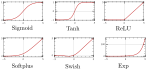
\includegraphics[width=0.8\columnwidth]{Figures/ActFunctions}
\caption{Activation functions used in ANNs.}
\label{fig:ActFunctions}
\end{figure}

The Sigmoid activation function~\cite{Han-1995-ISF}, also known as the logistic activation function, is widely used in ANNs.
It was originally developed in the field of logistic regression and later adapted for use in neural networks.
It maps any input to an output in the range~$[0,1]$, making it suitable for tasks where the network's output needs to represent probabilities or values between 0 and 1.
The Sigmoid activation function~$f(x)$ and its derivative~$f'(x)$ are defined by:
\begin{equation}
f(x) = \frac{1}{1+\e{-x}}\qquad \text{and}\qquad f'(x) = f(x)\cdotp\left[1-f(x)\right].\label{eq:act-sig}
\end{equation}
This function has been widely used until the early 1990s.
Its main advantage is that it is bounded, while its main drawbacks are the problem of vanishing gradient, a non-centered on zero output and saturation for large input values.

From 1990s to 2000s, the hyperbolic tangent activation function has been introduced and was preferred to the Sigmoid function for the training of ANNs.
The hyperbolic tangent function squashes the output within the range~$[-1,+1]$ and its formulation is given by the following equations:
\begin{equation}
f(x) = \frac{\e{x} - \e{-x}}{\e{x} + \e{-x}}\qquad \text{and}\qquad f'(x) = 1 - f(x)^2.\label{eq:act-tanh}
\end{equation}
This function is useful when the network needs to model data with mean-centered features, as it can capture both positive and negative correlations.
The Tanh activation function and the Sigmoid activation function are closely related in the sense that they both introduce non-linearity and squash their inputs into bounded ranges.
The evaluation of this activation function requires more CPU time than the Sigmoid function since we need to compute two exponential functions ($\e{x}$ and $\e{-x}$) to evaluate~$f(x)$.

ReLU is a classic function in classification ANNs due to its simplicity and computational efficiency, as it involves simple thresholding.
It introduces non-linearity and is computationally efficient.
It outputs the input if it's positive and zero if it's negative:
\begin{equation}
f(x) = \max(0,x)\qquad \text{and}\qquad f'(x) =
\begin{cases}
1&x>0\\
0&x\le 0
\end{cases}.\label{eq:act-relu}
\end{equation}
ReLU mitigates the vanishing gradient problem better than Sigmoid and Tanh, making it suitable for deep networks.
It often leads to faster convergence in training deep neural networks.
The vanishing gradient for all negative input is the major drawback of the ReLU function.

The Softplus function~\cite{Dugas-2000-ISO} approximates the ReLU activation function smoothly.
It is defined as the primitive of the Sigmoid function and is written:
\begin{equation}
f(x) = \log\left(1+\e{x}\right)\qquad \text{and}\qquad f'(x) = \frac{1}{1+\e{-x}}.\label{eq:act-softplus}
\end{equation}
Softplus activation function enhances a more gradual transition from zero than ReLU, and can model positive and negative values.
The main drawback is that its computational efficiency is low since we need to compute two exponential and one logarithmic functions to evaluate $f(x)$ and its derivative.

Swish~\cite{Ramachandran-2018-SAF} is a smooth and differentiable activation function defined as:
\begin{equation}
f(x) = \frac{x}{1+\e{-x}}\qquad \text{and}\qquad f'(x) = f(x) + \frac{1 - f(x)}{1+\e{-x}}.\label{eq:act-swish}
\end{equation}
Swish demonstrates enhanced performance in certain network architectures, particularly when employed as an activation function in deep learning models, and its simplicity and similarity to ReLU facilitate straightforward substitution in neural networks by practitioners.
%Swish has shown improved performance in some network architectures, especially when used as an activation function in deep learning models.
%The simplicity of Swish and its similarity to ReLU make it easy for practitioners to replace ReLUs with Swish units in any neural network.
Even if the expression of the Swish function and its derivative seems more complex that the Softplus function presented earlier, the CPU time is lower.

Looking at the shape of the ReLU and Swish functions, apart from those classic activations functions already widely used in ANNs, we propose here-after to add an extra one, based on the exponential function and simply defined by:
\begin{equation}
f(x) = \e{x}\qquad \text{and}\qquad f'(x) = f(x).\label{eq:act-exp}
\end{equation}
We found very few literature papers about the use of the exponential activation function in ANN, but it has been reported that in specific domains and mathematical modeling tasks, exponential activations can be highly relevant and effective.
The idea here is to use the property so that the derivative expression is defined only by the function itself, as well as for the Sigmoid and Tanh, but with the simplest formulation.
This will reduce the CPU cost since we need to compute both the function and its derivative for our implementation in the FE code into a very CPU intensive subroutine, due to the explicit integration.

Of course there is no limitation to the use of alternative activation functions in ANNs and there exist some much more complicated such as the one proposed by Shen \eal~\cite{Shen-2021-NNA} which is a combination of a floor, an exponential and a step function.
Those authors have proved that a three hidden layer with this activation function can approximate any Hölder continuous function with an exponential approximation rate.

In order to compare the different activation functions, all six activations functions presented earlier will be used in the rest of this paper and efficiency, precision of the models and computational cost will be analyzed.

%----------------------------------------------------------------------------------
\subsubsection{Pre and post processing architecture}\label{subsubsec:ANN-pre}
%----------------------------------------------------------------------------------

As we are using activations functions that mitigate vanishing gradients for large values, it is essential to normalize the three inputs and the output within the range of~$[0,1]$ to prevent ill-conditioning of the neural network.
%As we are using activations functions enhancing vanishing gradients for large values, the three inputs as well as the output must be normalized within the range~$[0,1]$ to avoid ill-conditioning of the neural network.
This range has been chosen because we will use the Sigmoid activation function as one of the six proposed formulations, while this later squashed the output to the lowest range~$[0,1]$.

Concerning the inputs, the range $\Delta[~]$ and minimum $[~]_{0}$ values of the input quantities are very different according to the data presented in Section~\ref{sec:Introduction}.
In our case, the range and minimum values of the strain are~$\Delta\varepsilon=0.7$ and~$\varepsilon_{0}=0$ respectively.
Concerning the strain rate~$\Delta\mdot{\varepsilon}=4.999~\ps$ and~$\mdot{\varepsilon}_{0}=0.001~\ps$ and concerning the temperature~$\Delta T=200~\celsius$ and~$T_{0}=1050~\celsius$.

As introduced in Pantalé \eal~\cite{Pantale-2021-EIN}, and with regard to considerations concerning the influence of the strain rate over the evolution of the stress, we first substitute~$\log(\mdot{\varepsilon}/\mdot{\varepsilon}_{0})$ for~$\mdot{\varepsilon}$.
Then in a second time, we remap the inputs $x_i$ within the range~$[0,1]$, so that the input vector~$\overrightarrow{x}$ is calculated from $\varepsilon$, $\mdot{\varepsilon}$ and $T$ using the following expressions:
\begin{equation}
\overrightarrow{x}=
\begin{cases}
x_{1} = \left(\varepsilon - \varepsilon_{0}\right)/\Delta\varepsilon \\
x_{2} = \left(\log(\mdot{\varepsilon}/\mdot{\varepsilon}_{0})-[\log(\mdot{\varepsilon}/\mdot{\varepsilon}_{0})]_{0}\right)/\Delta[\log(\mdot{\varepsilon}/\mdot{\varepsilon}_{0})]\\
x_{3} = \left(T-T_{0}\right)/\Delta T
\end{cases},
\label{eq:ANN-input}
\end{equation}
where~$[~]_{0}$ and~$\Delta[~]$ are the minimum and range values of the corresponding field.

The flow stress~$\sigma$, enhances the same behavior with~$\Delta\sigma=153.7~\MPa$ and~$\sigma_{0}=0~\MPa$.
Therefore, we apply the same procedure as previously presented and the flow stress~$\sigma$ is related to the output~$s$ according to the expression:
\begin{equation}
\sigma = \Delta\sigma.s + \sigma_{0}.\label{eq:ANN-output}
\end{equation}

%----------------------------------------------------------------------------------
\subsubsection{Derivatives of the Neural Network}\label{subsubsec:ANN-der}
%----------------------------------------------------------------------------------

As presented in Section~\ref{sec:Introduction}, in order to implement the ANN as a Fortran routine in Abaqus, we need to compute the three derivatives of $\sigma$ with respect to t$\varepsilon$, $\mdot{\varepsilon}$ and $T$.
We can compute those derivatives using differentiation of the output with respect to the inputs.
As illustrated in Figure~\ref{fig:ANN-2HL}, we are using here a two hidden layers neural network.
Therefore, as Equations (\ref{eq:ANN-y}-\ref{eq:ANN-s}) are used to compute~$\overrightarrow{y}\lay{k}$ and~$\overrightarrow{\hat{y}}\lay{k}$ for each hidden layer and the output~$s$ from the input vector~$\overrightarrow{x}$ of the ANN we can write the derivative~$\overrightarrow{s}'$ of a two hidden layers network as follow:
\begin{equation}
\overrightarrow{s}' = \w\lay{1}^T \dotp\left[\left(\w\lay{2}^T \dotp \left(\overrightarrow{w}^T \circ f'(\overrightarrow{y}\lay{2})\right)\right) \circ f'(\overrightarrow{y}\lay{1})\right] \label{eq:ANN-der},
\end{equation}
where~$f'\left(\square\right)$ is the activation function's derivative introduced by Equations (\ref{eq:act-sig}-\ref{eq:act-exp}) and~$\circ$ is the Hadamard product (the so called element-wise product).
Because of the pre and post processing of the values introduced in Section~\ref{subsubsec:ANN-pre}, the derivative of the flow stress~$\sigma$ with respect to the inputs~$\varepsilon$, $\mdot{\varepsilon}$ and~$T$ is then given by:
\begin{equation}
\begin{cases}
\partial \sigma/\partial \varepsilon = s'_{1}.\Delta\sigma / \Delta\varepsilon\\
\partial \sigma/\partial\mdot{\varepsilon} = s'_{2}.\Delta\sigma / (\mdot{\varepsilon}.\Delta\mdot{\varepsilon})\\
\partial \sigma/\partial T = s'_{3}.\Delta\sigma / \Delta T
\end{cases}
\label{eq:ANN-der2},
\end{equation}
where~$s'_i$ is one of the three components of the vector~$\overrightarrow{s}'$ defined by Equation (\ref{eq:ANN-der}).

Finally, Equations (\ref{eq:ANN-y}-\ref{eq:ANN-s}), (\ref{eq:ANN-input}-\ref{eq:ANN-der2}) and the requested activation function defined by one of the Equations (\ref{eq:act-sig}-\ref{eq:act-exp}) will be used to implement the ANN as a Fortran subroutine for the Abaqus FE software as it will be presented in Section~\ref{subsec:Num-impl}.

%----------------------------------------------------------------------------------
\subsection{Training of the ANN on experimental data}\label{subsec:train}
%----------------------------------------------------------------------------------

The Python program, developed with the dedicated library Tensorflow~\cite{Tensorflow-2015}, utilized the Adaptive Moment Estimation (ADAM) optimizer~\cite{Kingma-2015-AMS} and the Mean Square Error for assessing the loss function during the training phase.
%The Python program used for training the neural network was created with the dedicated Python library, Tensorflow~\cite{Tensorflow-2015}.
%The training phase employed the Adaptive Moment Estimation (ADAM) optimizer~\cite{Kingma-2015-AMS} and the Mean Square Error to evaluate the loss function.
With regard to our previous publications about ANN constitutive flow law~\cite{Pantale-2021-EIN}, we have made the choice to arbitrary fix some hyper-parameters of the ANNs, so to use a two hidden layers ANN with 15 neurons for the first hidden layer and 7 neurons for the second hidden layer.
There is a total number of~$180$ trainable parameters to optimize.
As we have 3 inputs and 1 output, we reference each of the ANNs using the notation 3-15-7-1-act, where act refers the activation function used for the model.
All six models underwent parallel training for a consistent number of iterations ($6~000$ iterations, lasting around 1 hour), on a PowerEdge R730 server running Ubuntu 22.04 LTS 64-bit, equipped with 96 GB of RAM and 2 Intel Xeon CPU E5-2650 2.20GHz processors.

Concerning the dataset used for the training of the ANN, as already introduced in the previous sections, this dataset is composed of~$21~030$ quadruplets ($\varepsilon$, $\mdot{\varepsilon}$, $T$ and~$\sigma$) acquired during the Gleeble experiments described in Section \ref{subsec:ExpTests}.
A chunk of $75\%$ of the dataset is used for training while the rest is used for the test during the training of the ANN.
All details about this procedure can be found in Pantalé~\cite{Pantale-2023-SSF} where the interested reader can download the source, data and results of this training program.
Regarding the training procedure, specifically the starting point, all models are initialized with precisely identical weights and biases.
However, due to different activation functions, the initial solution varies from one model to another.

Error evaluation of the models uses the Mean Square Error ($\MSE$), the Root Mean Square Error ($\RMSE$) and the Mean Absolute Relative Error ($\MARE$) given by the following equations:
\begin{equation}
\begin{cases}
\MSE = \frac{1}{N} \sum_{i=1}^{N} \left(\square_i^e - \square_i\right)^2\\
\RMSE (\MPa) = \sqrt{\MSE}\\
\MARE(\%) = \frac{1}{N} \sum_{i=1}^{N}{\left|\frac{\square_i -\square_i^e}{\square_i^e}\right|} \times 100
\end{cases},
\label{eq:Errors}
\end{equation}
where~$N$ is the total number of points for the computation of those errors, $\square_i$ is the~$i$th output value of the ANN, and~$\square_i^e$ is the corresponding experimental value.

Figure~\ref{fig:ANN-conv} show the evolution of the common logarithm of the Mean Square Error, \ie $\log_{10}(\MSE)$, of the output $s$ of the ANN during the training, evaluated using only the test data ($25\%$ of the dataset).
\begin{figure}[h!]
\centering
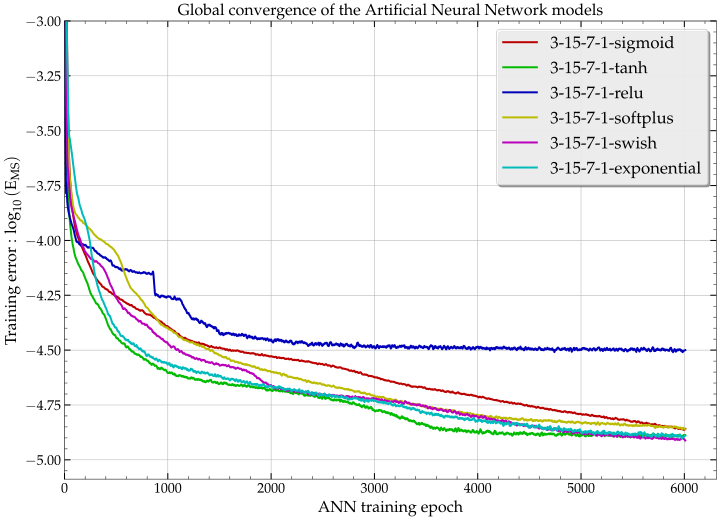
\includegraphics[width=0.7\columnwidth]{Figures/3Cr2Mo-convergence}
\caption{Global convergence of the six ANN models.}
\label{fig:ANN-conv}
\end{figure}
By examining this figure, we can assess and compare the convergence rates of various ANNs, concluding that a stable state was more or less achieved for all analyzed ANNs after $6~000$ iterations.
As expected, the ReLU activation function gives the worst results with a final value of~$\MSE=32\times10^{-6}$, mainly due to the low number of neurons and the fact that this function is a piecewise linear function and not able to efficiently approximate the nonlinear behavior of the material.
The other five activation functions enhance more or less the same behavior.
The final value of the $\MSE$ is pretty much the same for all of them, and around $\MSE=12\times10^{-6}$.
%The Tanh Swish, and Exp activation functions are slightly less powerful than the Sigmoid, and Softplus functions.
Table~\ref{tab:Training} reports the results of the training phase, the errors reported in this Table are computed using the whole dataset (both train and test parts).
\begin{table}[h!]
\caption{Comparison of the models' error depending on the activation function used.\label{tab:Training}}
\begin{tabular}{l|c|c|cc|cc|cc}
\toprule
Activation & CPU & $\MSE$ & $\RMSE$ & $\Delta\RMSE$ & $\MARE$ & $\Delta\MARE$ &  $\Delta E$ & rank \\
 & & $\times 10^{-6}$ & (\MPa) & & (\%) & & &\\ \midrule
Sigmoid & 1:04 & 13.853 & 0.604 & 1.007 & 1.412 & 1.201 & 1.536 & 2\\
Tanh & 1:03 & 12.890 & 0.621 & 1.035 & 1.634 & 1.390 & 1.748 & 5\\
ReLU & 1:03 & 31.537 & 0.860 & 1.434 & 2.750 & 2.339 & 2.881 & 6\\
Softplus & 1:04 & 13.968 & 0.600 & / & 1.617 & 1.375 & 1.724 & 4\\
Swish & 1:04 & 12.434 & 0.619 & 1.417 & 0.720 & 1.205 & 1.546 & 3\\
Exp & 1:03 & 12.843 & 0.688 & 1.147 & 1.176 & / & 1.362 & 1\\
\bottomrule
\end{tabular}
\end{table}

From the data, it is evident that all models require approximately the same training time to complete the specified number of iterations, with the complexity of activation functions influencing this duration; notably, the training time is a bit greater for Swish and Softplus functions compared to ReLU.
We also reported in this table the real values of the~$\RMSE$ and~$\MARE$ concerning the flow stress~$\sigma$ using the whole experimental database.
From this later we can see that the~$\RMSE$ is about~$0.6~\MPa$ for all activation functions except the ReLU one where the value is above~$0.8~\MPa$.
Concerning the $\MARE$, the value of all models is around~$1\%$ while it is more than~$2\%$ for the ReLU function.
Of the six activation functions, the Exponential function gives the best results in terms of solution quality, while the ReLU function gives the worst, as reported by computing the global error using the following expression $\Delta E=\sqrt{\RMSE^2+\MARE^2}$.
But we must note that the results of all models, except the ReLU one are very close at the end of the training stage, as illustrated in Figure~\ref{fig:ANN-conv} and Table~\ref{tab:Training}.
Depending on when the train is stopped, a particular model may yield the best performance due to the varying slopes of convergence among the models.
%From another point of view, the Swish activation function requires the most training time, but the difference is not discriminatory given the performance at this stage of the study.

Figure~\ref{fig:ANNFit} reports a comparison of the experimental stress acquired during the Gleeble compression tests (reported as dots in Figure~\ref{fig:ANNFit}) and the predicted stress~$\sigma$ using the ANN for the strain rate~$\mdot{\varepsilon}=1~\ps$.
\begin{figure}[h!]
\centering
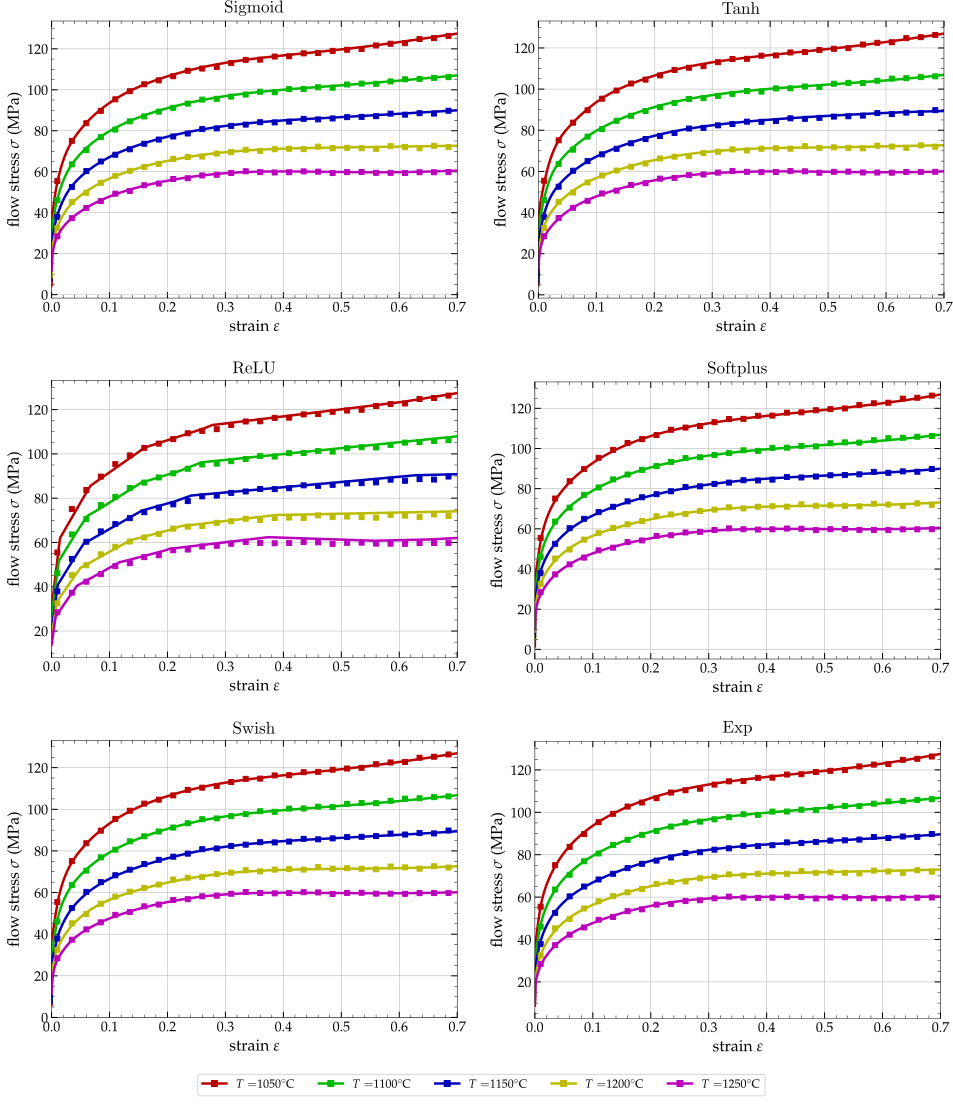
\includegraphics[width=0.95\columnwidth]{Figures/ANN-fit}
\caption{Comparison of experimental (dots) and the flow stress~$\sigma$ predicted by the ANN (continuous line) for~$\mdot{\varepsilon}=1~\ps$.}
\label{fig:ANNFit}
\end{figure}
From this observation, we can infer that all ANNs effectively replicate the experimental results, except for the ReLU activation function.
In the case of ReLU, as depicted in Figure~\ref{fig:ANNFit}, the predicted flow stress exhibits a piecewise linear behavior.

Of the six activation functions introduced, as detailed in Section~\ref{subsubsec:ANN-act}, the exponential function stands out due to its unique feature.
The computation of the function and its derivative in a single step necessitates only one evaluation of the exponential function, as indicated by $f'(x)=f(x)$ in Equation (\ref{eq:act-exp}).
If we analyze the results reported in Table~\ref{tab:Training} and Figure~\ref{fig:ANNFit} concerning the exponential activation function, we can see that this one has a $\RMSE=0.688~\MPa$, $\MARE=1.176\%$ and the global behavior of the flow stress for~$\mdot{\varepsilon}=1~\ps$ is similar to the Sigmoid, Tanh, Swish or Softplus functions.

In terms of global performance of the 3-15-7-1-exp ANN, Figure~\ref{fig:ANN-ExpFit} reports the comparison of the experimental data (dots) and the ANN flow stress for all strain rates and temperatures defined in Section~\ref{subsec:ExpTests}.
\begin{figure}[h!]
\centering
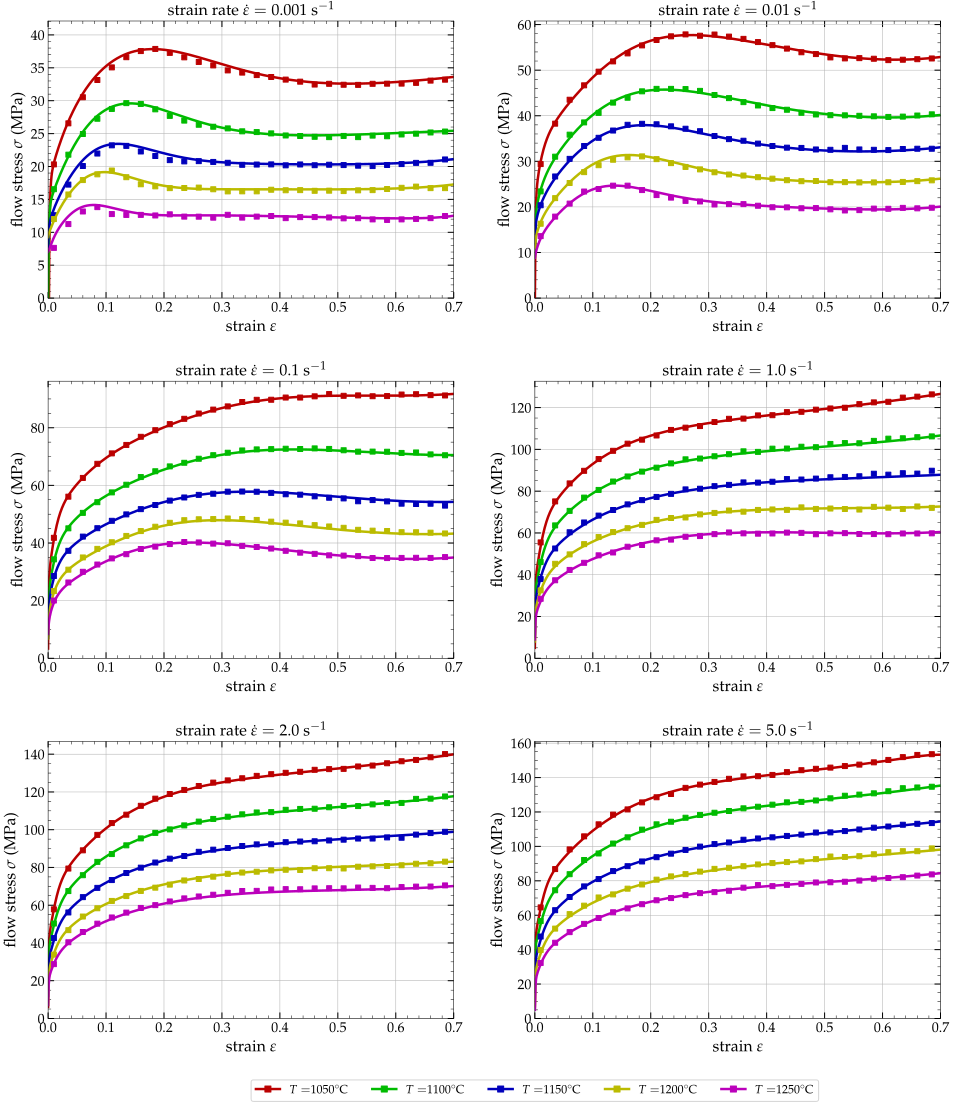
\includegraphics[width=0.95\columnwidth]{Figures/3Cr2Mo-3-15-7-1-exponential}
\caption{Comparison of experimental (dots) and ANN predicted flow stresses (continuous line) using the Exponential activation function.}
\label{fig:ANN-ExpFit}
\end{figure}
We can see that over the whole temperatures~$T$ and strain rates~$\mdot{\varepsilon}$, the performance of the model based on an exponential function is very good overall.
This model will therefore be retained for the remainder of the comparative study.

It is well known that artificial neural networks are able to interpolate data correctly within their learning domain, but behave unsatisfactorily when we wish to evaluate results outside the boundaries of this learning domain.
The ANNs developed in this study follow this general rule, but with different degrees of progress depending on the nature of the activation function used.
In order to test the extreme limits of the proposed networks, Figure~\ref{fig:ANN-Extrapolation} shows the comparison of predicted values according to the nature of the network for conditions globally outside the learning limits.
\begin{figure}[h!]
\centering
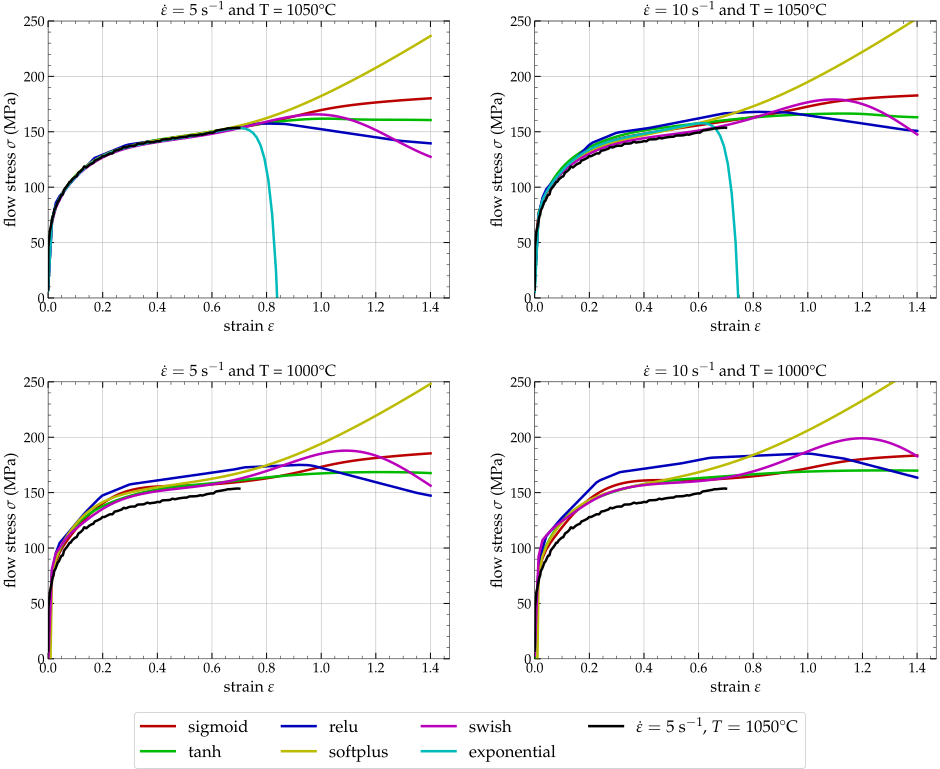
\includegraphics[width=0.95\columnwidth]{Figures/Extrapolation}
\caption{Comparison of the provided ANN results during an out of range computation.}
\label{fig:ANN-Extrapolation}
\end{figure}

We selected the worst case, multiplied the strain range by $2$ (up to $\varepsilon=1.4$), multiplied the strain rate by 2 ($\mdot{\varepsilon}=10$) and lowered the temperature to $T=1000\celsius$.
Figure~\ref{fig:ANN-Extrapolation} shows the evolution of the flow stress predicted by the six models.
In Figure~\ref{fig:ANN-Extrapolation}, top left, when deformation alone is extended, we can see that all six models correctly predict the flow stress evolution over the interval $\varepsilon=[0,0.7]$, whereas they diverge beyond a deformation of $\varepsilon=0.7$.
The behavior of the different models is highly variable, and overall, only the Sigmoid and Tanh models show a physically consistent trend.
The model with an exponential activation function behaves catastrophically outside the learning range, due to the very nature of the exponential function.
When deformation and temperature are out of range (top right), behavior is consistent below $\varepsilon=0.7$ and divergent beyond.
Again, only the Sigmoid and Tanh models show a physically consistent trend above $\varepsilon=0.7$.
When strain and strain rate are out of range (bottom left in Figure~\ref{fig:ANN-Extrapolation}), the behavior is consistent below $\varepsilon=0.7$, while diverging above $\varepsilon=0.7$.
The values given by the exponential model are out of range for all strain values.
Finally, when all inputs are out of range (bottom right), the behavior is consistent and identical except for the ReLU model below $\varepsilon=0.7$.
It is divergent above $\varepsilon=0.7$, and consistent only for the Sigmoid and Tanh models.

We can therefore conclude from this extrapolation study that it is important to remain as far as possible within the limits of the neural network's learning domain if the results are to be physically admissible.
Furthermore, from these analyses, it appears that only the Sigmoid and Tanh models are capable of physically admissible prediction of the flow stress values outside the learning domain.
This is due in particular to the double saturation of the tanh and sigmoid functions, as illustrated in Figure~\ref{fig:ActFunctions}, when the input values are outside the usual limits.

%----------------------------------------------------------------------------------
\section{Numerical simulations using the ANN flow law}\label{sec:Numerical}
%----------------------------------------------------------------------------------

Now that the flow stress models have been defined, trained and the results analyzed in terms of their relative performance in reproducing the experimental behavior recorded during compression tests on Gleeble, we will now numerically implement these models in Abaqus as a user routine in Fortran in order to perform numerical simulations.
Following training, the optimized internal parameters of the ANNs are saved in HDF5~\cite{Koranne-2011-HDF} files.
Subsequently, a Python program is responsible for reading these files and generating the Fortran 77 subroutine for Abaqus.

The implementation of a user flow law in Abaqus FE code, specifically using the Explicit version, involves programming the computation of the stress tensor $\Sig_{1}$ based on the stress tensor at the beginning of the increment $\Sig_{0}$ and the strain increment $\Delta\Eps$.
A predictor/corrector algorithm, such as the radial-return integration scheme~\cite{Ponthot-2002-USU}, is typically employed.
For detailed implementations, Ming \eal~\cite{Ming-2018-ERV} discusses the Safe-Newton integration scheme, and Liang \eal~\cite{Liang-2022} focuses on an application related to the Arrhenius flow law.
During the corrector phase, the flow stress $\sigma$ must be evaluated at the current integration point as a function of $\varepsilon$, $\mdot{\varepsilon}$, and $T$.
This process involves solving a non-linear equation defining the plastic corrector expression and computing three derivatives of the flow stress: $\partial\sigma/\partial\varepsilon$, $\partial\sigma/\partial\mdot{\varepsilon}$, and $\partial\sigma/\partial T$.
Typically, the subroutine VUHARD in the Abaqus explicit is responsible for computing these quantities, and its implementation depends on the structure and activation functions of the ANN.

%----------------------------------------------------------------------------------
\subsection{Numerical implementation of the ANN flow law}\label{subsec:Num-impl}
%----------------------------------------------------------------------------------

In order to have a better understanding of the implementation of the VUHARD subroutine, we are going to detail the computation of the flow stress and the three derivatives in one step as a function of the triplet of input values~$\varepsilon$, $\mdot{\varepsilon}$, $T$.
We suppose that the current input is stored in a three components vector $\overrightarrow{\xi}^T=\left[\varepsilon, \log(\mdot{\varepsilon}/\mdot{\varepsilon}_{0}), T\right]$.
We also suppose that the minimum and range values of the inputs, used during the learning phase, are stored in two vectors $\overrightarrow{\xi}_{0}$ and $\Delta\overrightarrow{\xi}$ respectively.
% The minimum and ran values of the stress are also stored in two variables $\sigma_{0}$ and $\sigma_{max}$ respectively.
\begin{itemize}
\item We first use Equation (\ref{eq:ANN-input}) to compute the vector $\overrightarrow{x}$ where all components of $\overrightarrow{\xi}$ will be remapped within the range $[0,1]$:
\begin{equation}
\overrightarrow{x}=\left(\overrightarrow{\xi}-\overrightarrow{\xi}_{0}\right)\oslash\Delta\overrightarrow{\xi}, \label{eq:ANNi1}
\end{equation}
where $\oslash$ is the Hadamard division operator.
\item Conforming to Equation (\ref{eq:ANN-y}), we compute the vector:
\begin{equation}
\overrightarrow{y}\lay{1}=\w\lay{1}\cdot\overrightarrow{x}+\overrightarrow{b}\lay{1}.\label{eq:ANNi2}
\end{equation}
\item Then, from Equation (\ref{eq:ANN-f}) and the expression of the activation function in the first layer and defined by one of the Equations (\ref{eq:act-sig}-\ref{eq:act-exp}), we compute the vector:
\begin{equation}
\overrightarrow{\hat{y}}\lay{1}=f\lay{1}(\overrightarrow{y}\lay{1}).\label{eq:ANNi3}
\end{equation}
\item We repeat the process for the second layer, so that we compute the vectors: \begin{equation}
\overrightarrow{y}\lay{2}=\w\lay{2}\cdot\overrightarrow{\hat{y}}\lay{1}+\overrightarrow{b}\lay{2},\label{eq:ANNi4}
\end{equation}
and:
\begin{equation}
\overrightarrow{\hat{y}}\lay{2}=f\lay{2}(\overrightarrow{y}\lay{2}).\label{eq:ANNi5}
\end{equation}
\item From Equations (\ref{eq:ANN-s}) and (\ref{eq:ANN-output}), we compute the flow stress $\sigma$ using the following equation:
\begin{equation}
\sigma = \Delta\sigma.\left(\overrightarrow{w}^T \dotp \overrightarrow{\hat{y}}\lay{2} + b\right) + \sigma_{0}.\label{eq:ANNi6}
\end{equation}
\item Then we can compute in a single step the three derivatives $\overrightarrow{\sigma}'$ from Equation (\ref{eq:ANN-der}) with the following expression:
\begin{equation}
\begin{array}{l}
\overrightarrow{\Sig}' = \Delta\sigma.\w\lay{1}^T \dotp\left[\left(\w\lay{2}^T \dotp \left(\overrightarrow{w}^T \circ f'(\overrightarrow{y}\lay{2})\right)\right) \circ f'(\overrightarrow{y}\lay{1})\right] \oslash \Delta\overrightarrow{\xi}\\
\Sig_{2}' := \Sig_{2}' / \mdot{\varepsilon}
\end{array},\label{eq:ANNi7}
\end{equation}
where the expression used for $f'()$ changes depending on the activation function used.
\end{itemize}
As an illustration the corresponding implementation using Python of those equations is proposed in Appendix \ref{sec:Appendix1}.
A dedicated Python program is used to translate those equations into a Fortran 77 subroutine.
During the translation phase, all functions corresponding to array operators, as matrix--matrix multiplications or element-wise operations, are converted into unrolled loops (explicitly written), all values of the ANNs parameters are explicitly written as data at the beginning of the subroutine, so that the a 3-15-7-1-exp Fortran routine consist of more than 400 lines of code.
A small extract of the corresponding VUHARD subroutine is presented in Figure~\ref{fig:FortranStress} in Appendix \ref{sec:Appendix2}.
All full source files of the six VUHARD subroutines is available in the Software Heritage Archive~\cite{Pantale-2023-SSF}.

The Fortran subroutine is compiled with double precision directive using the Intel Fortran 14.0.2 compiler on a Ubuntu 22.04 server and linked to the main Abaqus explicit executable.

%----------------------------------------------------------------------------------
\subsection{Numerical simulations and comparisons}\label{subsec:Num-sim}
%----------------------------------------------------------------------------------

To compare the influence of choosing different activation functions on the numerical results using Abaqus explicit, we have made the choice to model the compression test presented earlier in~\ref{subsec:ExpTests}.
We consider therefore a medium-carbon steel, type P20 cylinder in compression with the initial dimensions~$\phi_{0}=10$~mm and~$h_{0}=15$~mm as reported in Figure~\ref{fig:Num-model}, where only the superior half part of cylinder is represented, as the solution is symmetrical on either side of a cutting plane located halfway up the cylinder.
\begin{figure}[h!]
\centering
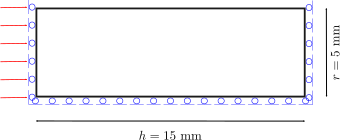
\includegraphics[width=0.25\columnwidth]{Figures/CyCompression}
\caption{Half axis-symmetric model for the numerical simulation of the compression of a cylinder.}
\label{fig:Num-model}
\end{figure}
At the end of the process, the height of the cylinder is~$h_f=9$~mm, \ie the top edge displacement is $d=6$~mm and the reduction is $40\%$ of the total height.
The displacement is applied with a constant speed and the simulation time is fixed to $t=1$~s, \ie the strain rate is in the range $\mdot{\varepsilon}=[0.5,1.0]~\ps$ at the center of the specimen.
%The six ANN flow laws will be compared here-after.
The mesh comprises 600 axis-symmetric thermomechanical quadrilateral finite elements (CAX4RT) featuring 4 nodes and reduced integration.
It includes 20 elements along the radial direction and 30 elements along the axis.
The element size is $0.25\times0.25~\text{mm}^2$.
Only reduced integration is available in Abaqus explicit for an axis-symmetric structure.
The anvils are modeled as two rigid surfaces and a Coulomb friction law with $\mu=0.15$ is used.
To reduce the computing time, a global mass scaling with a value of $M_s=1000$ is used.
The initial temperature of the material is set to $T_{0}=1150\celsius$, and we use an explicit adiabatic solver for the simulation of the compression process.
%The elastic properties of the material are fixed to a Young modulus $E=207~\GPa$ and a Poisson ration $\nu=0.285$.
%Conforming to the applied boundaries conditions used for the simulation of the compression test, and, the average strain rate during the compression for the center element of the specimen is around~$\mdot{\overline{\varepsilon}^p}=0.8~\ps$.
All simulations are performed using the 2022 version of the Abaqus explicit solver on the same computer as the one used for the learning of the ANNs in Section~\ref{subsec:train}.
Simulations are performed with the double precision version of the solver without any parallelization directive to better compare the CPU times.

Figure~\ref{fig:Num-peeqCP} shows, at the end of the simulation (when the displacement of the top edge is $d=6$~mm), a comparison of the equivalent plastic strain $\overline{\varepsilon}^p$ contourplot for the six activation functions.
\begin{figure}[h!]
\centering
\includegraphics[width=0.9\columnwidth]{Figures/PeeqHalf}
\caption{Equivalent plastic strain $\overline{\varepsilon}$ contourplot for the six activation functions.}
\label{fig:Num-peeqCP}
\end{figure}
%In this figure, only the top half of the cylinders is shown, as the solution is symmetrical on either side of a cutting plane located halfway up the cylinder.
From this later, we can clearly see that all activation functions gives almost the exact same results and the choice of any of the available ANN has no influence on the values and isovalues contourplot reported in Figure~\ref{fig:Num-peeqCP}.
%The slight difference in the scale of values for each case is due to the value of the plastic strain in the contact zone between the cylinder and the upper surface at the corner.
%As shown here after, the actual values for the central element of the specimen are virtually identical.
Figure~\ref{fig:Num-misesCP} shows a comparison of the von Mises equivalent stress $\overline{\sigma}$ contourplot.
\begin{figure}[h!]
\centering
\includegraphics[width=0.9\columnwidth]{Figures/MisesHalf}
\caption{Von Mises equivalent stress $\overline{\sigma}$ contourplot for the six activation functions.}
\label{fig:Num-misesCP}
\end{figure}
In this figure, we can see that the solutions differ slightly both in terms of maximum stress value and stress isovalues distribution.
%Nevertheless, the disparities in values remain minimal and below $1\%$ between the six different models.

In order to compare the different models quantitatively, Table~\ref{tab:Simulation} reports the values of the plastic strain $\overline{\varepsilon}^p$, the von Mises equivalent stress $\overline{\sigma}$ and the temperature $T$ for the element located at the center of the specimen at the end of the simulation.
\begin{table}[h!]
\caption{Comparison of quantitative results concerning the six activation functions analyzed.\label{tab:Simulation}}
\begin{tabular}{l|ccc|ccc}
\toprule
Activation & CPU & $N_{inc}$ & $N_{inc}$/s & $\overline{\varepsilon}^p$ & $\overline{\sigma}$ & $T$ \\
 & (s) & & & & (\MPa) &(\celsius)\\ \midrule
Sigmoid & 574 & 1~092~001 & 1902 & 0.762 & 87.6 & 1164.3 \\
Tanh & 648 & 1~096~099 & 1691 & 0.761 & 88.3 & 1164.4 \\
ReLU & 460 & 1~082~453 & 2353 & 0.750 & 85.6 & 1163.9 \\
Softplus & 906 & 1~087~812 & 1200 & 0.753 & 87.4 & 1164.1 \\
Swish & 738 & 1~082~832 & 1467 & 0.753 & 86.6 & 1164.0 \\
Exp & 540 & 1~077~954 & 1996 & 0.757 & 85.6 & 1164.1 \\
\bottomrule
\end{tabular}
\end{table}
From the values reported in this Table, we can see that the models differ a little concerning the equivalent stress (below $1\%$), the equivalent plastic strain (below $1\%$) and the temperature (below $0.02\%$).
%In fact the Sigmoid, Tanh and Exp activation functions give almost the same results concerning the plastic strain and temperature results.
It is important to note that one origin of the differences between the models comes from the fact that in the end of the simulation, the plastic strain $\overline{\varepsilon}^p$ is greater than $0.7$, so the model has to extrapolate the yield stress with respect to the data used for the training phase.
This increases the discrepancy between the models, since each extrapolates the results from the training domain differently with respect to its internal formulation.

In Table~\ref{tab:Simulation} we also have reported the number of increments $N_{inc}$ needed to complete the simulation along with the total CPU time.
We remark that the number of increment varies from one activation function to another one, since the convergence of the model differ because it takes into account the stress in the computation of the stable time increment.
From these two, we can calculate the number of increments performed per second and propose a classification from the fastest to the slowest ANN, where: ReLU is the fastest (with 2353 iteration per second) and Softplus is the slowest (with 1200 iteration per second) of the proposed models (two times slower than the ReLU one).
Those results are directly linked to the complexity of the expression of the activation function and its derivative as introduced in Section~\ref{subsubsec:ANN-act}.
For example, we can note that a simulation using the Sigmoid activation function requires 1~092~001 increments and the model contains 400 under integrated CAX4RT elements, therefore, we will have 436~800~400 computations of the code presented in Figure~\ref{fig:FortranSigmoid}.
From those results, we can note that, as expected, the Exp activation function is very efficient in terms of CPU computation time (with 1996 iteration per second) as it is just second after the very light ReLU function, but gives quite good results as reported in Table~\ref{tab:Simulation} which is not the case of the ReLU function.

Figure~\ref{fig:Num-misesTH} shows the evolution of the von Mises stress vs. displacement of the top edge for the center of the cylinder for all activation functions.
\begin{figure}[h!]
\centering
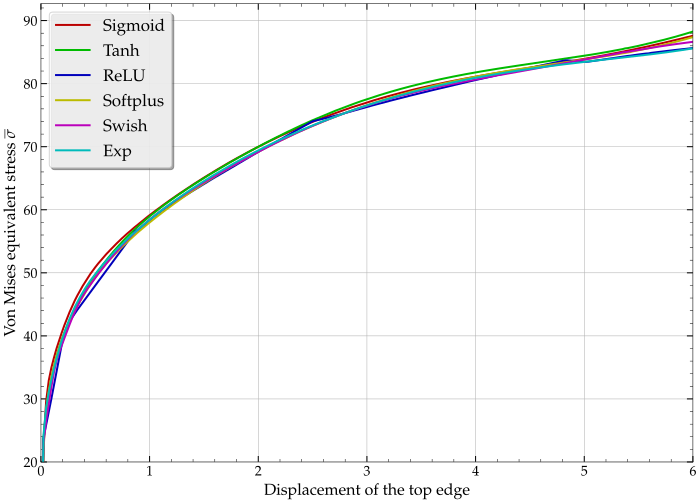
\includegraphics[width=0.7\columnwidth]{Figures/vonMises}
\caption{Von Mises stress vs. displacement of the top edge of the cylinder for all activation functions.}
\label{fig:Num-misesTH}
\end{figure}
%The other three activations functions enhancing the same behavior as the Exp and Sigmoid ones %have been removed to simplify the graph.
From this later, we can see that all activation functions give almost the same results, while the ReLU enhances a piecewise behavior due to its formulation and the low number of neurons used for the ANN.
This behavior has an influence on the precision of the ANN flow law, and we suggest avoiding the use of the ReLU activation function in this kind of application.
Any other type of activation function give quite good results for this application, while among them, the use of the Exp activation function gives accurate results and minimum computation time for numerical applications.

%----------------------------------------------------------------------------------
\section{Conclusions and major remarks}\label{sec:Conclusions}
%----------------------------------------------------------------------------------

In this paper, several ANN based flow laws for thermomechanical simulation of the behavior of a P20 medium-alloy steel have been identified.
These six laws exhibit distinctions solely in the choice of their activation functions, while maintaining a uniform architectural framework characterized by consistent specifications regarding the quantity of hidden layers and the number of neurons present on each of these hidden layers.
In addition to the five classic activation functions (Sigmoid, Tanh, ReLU, Softplus and Swift), we proposed the use, in this paper, of the Exp (exponential) function as an activation function, although this is almost never used in neural network formulations.
The expressions of the activation functions and their derivatives were used in the neural network writing formalism to calculate the derivatives of~$\sigma$ with respect to~$\varepsilon$, $\mdot{\varepsilon}$ and~$T$.

Comparison of the ANNs results (in terms of flow stress $\sigma$) with experiments have shown that all five activation functions, with the exception of the ReLU function, give very good results, far superior to those obtained conventionally using formalisms based on analytical flow laws from the literature, such as the Johnson--Cook, Arrhenius or Zerilli--Armstrong models~\cite{Tize-2023-IEP}.
To improve the extrapolation ability of the models, it is recommended to use the Sigmoid and Tanh activation functions.
These functions can effectively squash out of bounds values, giving the artificial neural network a more realistic behavior beyond the training bounds.

Based on the equations describing the mathematical formulation of an ANN with two hidden layers, and depending on the nature of these activation functions, we have implemented these constitutive laws in the form of a Fortran 77 subroutine for Abaqus explicit.
The same approach can also be used to write a UHARD routine enabling the same flow laws to be used in Abaqus standard.

Numerical results obtained from a compression test on a metal cylinder using the Abaqus explicit code have shown that neural network behavior models give very satisfactory results, in line with experimental tests.
The Exp activation function, which is rarely used in the formulation of artificial neural networks, showed very good results (in agreement with more complex models such as Tanh), while enabling the code user to benefit from the efficiency and ease of implementation of an exponential function.
These results are satisfactory insofar as the inputs remain entirely within the model's learning domain, since the extrapolation capabilities of the network based on the exponential function are very limited.
We then obtain results equivalent in terms of solution quality to sigmoid or tanh-type formulations, while having computation times comparable to a ReLU function.

Overall, this study concludes by recommending the use of the sigmoid activation function for the development of flow laws, since it gives very good results in the identification domain, allows us to leave the learning domain with a behavior that is certainly biased, but physically admissible, and offers very good performance in terms of simulation time when implemented in a finite element code.
This study emphasizes the valuable impact of neural network-derived flow laws for numerical finite element simulation executed with a commercial FE code like Abaqus.

%%%%%%%%%%%%%%%%%%%%%%%%%%%%%%%%%%%%%%%%%%
%\section{Patents}


%%%%%%%%%%%%%%%%%%%%%%%%%%%%%%%%%%%%%%%%%%
\vspace{6pt}

%%%%%%%%%%%%%%%%%%%%%%%%%%%%%%%%%%%%%%%%%%
%% optional
%\supplementary{The following supporting information can be downloaded at: \linksupplementary{s1}, Figure S1: title; Table S1: title; Video S1: title.}

% Only for the journal Methods and Protocols:
% If you wish to submit a video article, please do so with any other supplementary material.
% \supplementary{The following supporting information can be downloaded at: \linksupplementary{s1}, Figure S1: title; Table S1: title; Video S1: title. A supporting video article is available at doi: link.}

%%%%%%%%%%%%%%%%%%%%%%%%%%%%%%%%%%%%%%%%%%
%\authorcontributions{
%All authors have read and agreed to the published version of the manuscript.}

\funding{This research received no external funding.}

%\institutionalreview{In this section, you should add the Institutional Review Board Statement and approval number, if relevant to your study. You might choose to exclude this statement if the study did not require ethical approval. Please note that the Editorial Office might ask you for further information. Please add “The study was conducted in accordance with the Declaration of Helsinki, and approved by the Institutional Review Board (or Ethics Committee) of NAME OF INSTITUTE (protocol code XXX and date of approval).” for studies involving humans. OR “The animal study protocol was approved by the Institutional Review Board (or Ethics Committee) of NAME OF INSTITUTE (protocol code XXX and date of approval).” for studies involving animals. OR “Ethical review and approval were waived for this study due to REASON (please provide a detailed justification).” OR “Not applicable” for studies not involving humans or animals.}

%\informedconsent{Any research article describing a study involving humans should contain this statement. Please add ``Informed consent was obtained from all subjects involved in the study.'' OR ``Patient consent was waived due to REASON (please provide a detailed justification).'' OR ``Not applicable'' for studies not involving humans. You might also choose to exclude this statement if the study did not involve humans.
%
%Written informed consent for publication must be obtained from participating patients who can be identified (including by the patients themselves). Please state ``Written informed consent has been obtained from the patient(s) to publish this paper'' if applicable.}

\dataavailability{Source files of the numerical simulations and the ANN flow laws are available from~\cite{Pantale-2023-SSF}.}

\acknowledgments{The author thanks the team of Pr. Mohammad Jahazi from the Ecole Technique Supérieure de Montréal, Canada, for providing the experimental data used in Section~\ref{subsec:ExpTests}.}

\conflictsofinterest{The author declare no conflict of interest.}

%%%%%%%%%%%%%%%%%%%%%%%%%%%%%%%%%%%%%%%%%%
%% Optional
%\sampleavailability{Samples of the compounds ... are available from the authors.}

%% Only for journal Encyclopedia
%\entrylink{The Link to this entry published on the encyclopedia platform.}

\abbreviations{Abbreviations}{
The following abbreviations are used in this manuscript:\\

\noindent
\begin{tabular}{@{}ll}
ANN & Artificial Neural Network \\
CAX4RT & Abaqus 4 nodes axis-symmetric thermomechanical element \\
CPU & Central processing unit \\
FE & Finite Element \\
UHARD & Abaqus standard user subroutine \\
VUHARD & Abaqus explicit user subroutine \\

\end{tabular}
}

%%%%%%%%%%%%%%%%%%%%%%%%%%%%%%%%%%%%%%%%%%
%% Optional
\appendixtitles{yes} % Leave argument "no" if all appendix headings stay EMPTY (then no dot is printed after "Appendix A"). If the appendix sections contain a heading then change the argument to "yes".
\appendixstart
\appendix

%----------------------------------------------------------------------------------
\section[\appendixname~\thesection]{Python code to compute stress and derivatives\label{sec:Appendix1}}
%----------------------------------------------------------------------------------

The implementation using Python of Equations (\ref{eq:ANNi1}) to (\ref{eq:ANNi7}) is proposed in Figure~\ref{fig:PythonStress}, where the arguments of the function \var{stressAndDerivatives} are \var{xi} for the~$\overrightarrow{\xi}$ vector, \var{deps} for~$\mdot{\varepsilon}$, \var{Act} for the activation function and \var{dAct} for its derivative.
\begin{figure}[h!]
\begin{PythonListing}
def stressAndDerivatives(xi, deps, Act, dAct):
  x = (xi - xi0) / Dxi
  y1 = w1.dot(x) + b1
  yf1 = Act(y1)
  y2 = w2.dot(yf1) + b2
  yf2 = Act(y2)
  Sig = Dsig*(w.dot(yf2) + b) + sig0
  dSig = Dsig*((w1.T).dot((w2.T).dot(w.T*dAct(y2))*dAct(y1))) / Dxi
  dSig[1] = dSig[1] / deps
  return Sig, dSig
\end{PythonListing}
\caption{Python function to compute the flow stress and the derivative vector.\label{fig:PythonStress}}
\end{figure}
The network architecture is defined by the numpy arrays \var{w1}, \var{w2}, \var{w}, \var{b1}, \var{b2} and \var{b} which are global variables in the proposed piece of code.
The other variables \var{xi0}, \var{Dxi}, \var{sig0} and \var{Dsig} correspond to the quantities~$\overrightarrow{\xi}_{0}$, $\Delta\overrightarrow{\xi}$, $\sigma_{0}$ and $\Delta\sigma$ respectively.

Line~2 in Figure~\ref{fig:PythonStress} correspond to Equation (\ref{eq:ANNi1}).
Lines~3 and~4 correspond to Equations (\ref{eq:ANNi2}) and (\ref{eq:ANNi3}) and concerns the first hidden layer, while lines~5 and~6 correspond to Equations (\ref{eq:ANNi4}) and (\ref{eq:ANNi5}) and concerns the second hidden layer.
Finally, line~7 computes the flow stress $\sigma$ conforming to Equation (\ref{eq:ANNi6}) and lines~8 and~9 computes the three derivatives of the flow stress conforming to Equation (\ref{eq:ANNi7}).
The stress \var{Sig} and the three derivatives array \var{dSig} are returned as a tuple at line~10.

%----------------------------------------------------------------------------------
\section[\appendixname~\thesection]{Fortran 77 subroutines to implement the ANN flow law\label{sec:Appendix2}}
%----------------------------------------------------------------------------------

A portion of the Fortran 77 code defining the numerical implementation of the VUHARD routine for Abaqus Explicit is presented in Figure~\ref{fig:FortranStress}.
The complete source codes for the flow laws corresponding to the six activation functions can be found in the Software Heritage archive~\cite{Pantale-2023-SSF}.
In Figure~\ref{fig:FortranStress}, the '...' symbols denote a continuation of the code that is not transcribed here due to space constraints in the figure for the sake of conciseness.

\begin{figure}[!h]
\begin{FortranListing}
      subroutine vuhard (... Heading of VUHARD routine ...)
      ...
c Block of Data
      double precision w1(15, 3)
      data w1/-0.480648012140D0, 1.20722861399D0, -0.024459252119D0,
     + -0.088911109397D0,
      ...
c Preprocessing of the variables
      xeps = (eqps(k) - xmI(1))/xrI(1)
      xdeps = (log(eqpsRate(k)/xdeps0) - xmI(2))/xrI(2)
      xtemp = (tempNew(k) - xmI(3))/xrI(3)
c Hidden layer #1 (y11 to y115)
      y11 = w1(1,1)*xeps + w1(1,2)*xdeps + w1(1,3)*xtemp + b1(1)
      ...
c exponential activation function (yf11 to yf115)
      yf11 = exp(y11)
      ...
c Hidden layer #2 (y21 to y27)
      y21 = w2(1,1)*yf11 + w2(1,2)*yf12 + w2(1,3)*yf13
     + +w2(1,4)*yf14 + ... + b2(1)
      ...
c exponential activation function (yf21 to yf27)
      yf21 = exp(y21)
      ...
c Derivatives terms (xa1 to xa7), (xb1 to xb15)
      xa1 = w3(1)*yf21
      ...
      xb1 = (w2(1,1)*xa1 + w2(2,1)*xa2 + w2(3,1)*xa3
     + +w2(4,1)*xa4 + ... + w2(7,1)*xa7)*yf11
      ...
c Outputs of the subroutine
      Yield(k) = xrO*(w3(1)*yf21 + w3(2)*yf22
     + +w3(3)*yf23 + ... + b3) + xmO
      dyieldDeqps(k,1) = xrO*(w1(1,1)*xb1 + w1(2,1)*xb2
     + +w1(3,1)*xb3 + ... + w1(15,1)*xb15) / xrI(1)
      dyieldDeqps(k,2) = xrO*(w1(1,2)*xb1 + w1(2,2)*xb2
     + +w1(3,2)*xb3 + ... + w1(15,2)*xb15)/(xrI(2)*eqpsRate(k))
      dyieldDtemp(k) = xrO*(w1(1,3)*xb1 + w1(2,3)*xb2
     + +w1(3,3)*xb3 + ... + w1(15,3)*xb15) / xrI(3)
c Return from the VUHARD subroutine
      return
      end
\end{FortranListing}
\caption{Part of the VUHARD Fortran 77 subroutine for the ANN flow law and the exponential activation function.\label{fig:FortranStress}}
\end{figure}
Depending on the kind of activation function used, some lines differ from one version to the other one, such as the definitions of the activation functions (see line 16 in Figure~\ref{fig:FortranStress}) and the expressions of the internal variables \var{xa} and \var{xb} (see lines 26 and 28 in Figure~\ref{fig:FortranStress}).

Figure~\ref{fig:FortranSigmoid} show the declaration of the Sigmoid activation function and its derivative as defined by Equation (\ref{eq:act-sig}), while Figure~\ref{fig:FortranSoftplus} show the same part of the code with the use of the Softplus activation function as defined by Equation (\ref{eq:act-softplus}).
\begin{figure}[h!]
\begin{FortranListing}
c sigmoid activation function (yf11 to yf115)
      yf11 = 1/(1 + exp(-y11))
      ...
c Derivatives terms (xa1 to xa7), (xb1 to xb15)
      xa1 = w3(1)*(yf21*(1 - yf21))
      ...
      xb1 = (w2(1,1)*xa1 + w2(2,1)*xa2 + w2(3,1)*xa3
     + +w2(4,1)*xa4 + ... + w2(7,1)*xa7)*(yf11*(1 - yf11))
      ...
\end{FortranListing}
\caption{Part of the VUHARD Fortran 77 subroutine with the Sigmoid activation function.\label{fig:FortranSigmoid}}
\end{figure}
\begin{figure}[h!]
\begin{FortranListing}
c softplus activation function (yf11 to yf115)
      yf11 = log(1 + exp(y11))
      ...
c Derivatives terms (xa1 to xa7), (xb1 to xb15)
      xa1 = w3(1)*(1/(1 + exp(-y21)))
      ...
      xb1 = (w2(1,1)*xa1 + w2(2,1)*xa2 + w2(3,1)*xa3
     + +w2(4,1)*xa4 + ... + w2(7,1)*xa7)*(1/(1 + exp(-y11)))
      ...
\end{FortranListing}
\caption{Part of the VUHARD Fortran 77 subroutine with the Softplus activation function.\label{fig:FortranSoftplus}}
\end{figure}

%%----------------------------------------------------------------------------------
%\section[\appendixname~\thesection]{ANN Flow Law Coefficients\label{sec:Appendix}}
%%----------------------------------------------------------------------------------
%
%In order to complete this paper, we report here after the computing process and the $180$~coefficients of the artificial neural network ANN-3-15-7-1-exp model.
%The weight matrix for the first hidden layer $\w_{1}$ is a $17\times3$ matrix:
%\begin{equation*}
%\w_{1} = \left[
%\begin{array}{rrr}
%-18.005 & 1.250 & -1.342\\
%-2.126 & 0.829 & -4.838\\
%-2.151 & 4.882 & -1.110\\
%-0.832 & -4.702 & 0.888\\
%1.348 & 1.259 & -1.429\\
%-0.397 & 2.798 & 0.710\\
%-8.646 & -5.529 & -3.916\\
%0.835 & 3.751 & -37.522\\
%0.362 & 0.118 & 8.211\\
%-6.782 & 1.091 & 0.319\\
%-0.386 & 0.794 & -1.934\\
%-0.030 & -4.024 & 0.773\\
%1.488 & -2.371 & 4.147\\
%-10.993 & -8.295 & -12.164\\
%-2.439 & -0.757 & -0.323\\
%-280.787 & 1.176 & -0.090\\
%-3.538 & -2.779 & -19.796\\
%\end{array}\right]
%\end{equation*}
%
%The biases of the first hidden layer $\overrightarrow{b_{1}}$ is a $17$-component vector:
%\begin{equation*}
%\overrightarrow{b}_{1} = \left[
%\begin{array}{r}
%-0.610\\
%-2.237\\
%-4.040\\
%1.134\\
%-3.054\\
%-3.478\\
%1.501\\
%-5.838\\
%-8.602\\
%-1.245\\
%-1.556\\
%0.738\\
%-5.335\\
%2.208\\
%-0.629\\
%-1.619\\
%-0.080\\
%\end{array}\right]
%\end{equation*}
%
%The weight matrix for the second hidden layer $\w_{2}$ is a $9\times17$ matrix:
%\begin{equation*}
%\w_{2}^T = \left[
%\begin{array}{rrrrrrrrr}
%0.133 & -86.946 & -1.051 & 1.803 & -1.850 & -0.440 & -7.127 & 0.174 & -0.340\\
%7.083 & -20.359 & 4.734 & 2.643 & 1.095 & -0.023 & -27.715 & -0.822 & -0.648\\
%-4.270 & -42.833 & -1.828 & -0.537 & 0.706 & 0.311 & -52.811 & 0.850 & -0.099\\
%-4.290 & 2.243 & -30.375 & 0.054 & 1.164 & -1.643 & -1.862 & 0.987 & -1.024\\
%-9.379 & -2.773 & 0.583 & -3.396 & -7.241 & -1.776 & -13.472 & 0.536 & -2.769\\
%-8.435 & -8.215 & 1.744 & 0.019 & 2.242 & 0.089 & -15.298 & -2.382 & -6.080\\
%8.050 & -3.032 & -10.094 & 0.164 & -3.551 & -0.090 & 4.431 & -1.937 & 3.075\\
%-33.193 & -1.846 & -2.293 & -2.618 & 16.397 & -1.025 & -2.828 & 1.294 & 6.319\\
%2.114 & 1.389 & -0.987 & -0.090 & -1.819 & -0.097 & 2.508 & 0.687 & 0.878\\
%-2.214 & -14.317 & -2.055 & 0.387 & 1.097 & -0.712 & 8.227 & -3.942 & -1.930\\
%-13.351 & 1.743 & 3.924 & -5.355 & -6.500 & 1.088 & 3.149 & -1.526 & -0.613\\
%-2.844 & -3.412 & -11.884 & 0.033 & -2.475 & -1.387 & 2.261 & -1.787 & -0.300\\
%-13.599 & -5.833 & 8.660 & 0.092 & -4.317 & 1.483 & -14.671 & -5.869 & 1.144\\
%-23.598 & 0.261 & 18.128 & -0.031 & -2.716 & -0.374 & -72.263 & 0.565 & -1.063\\
%2.988 & -3.510 & 5.437 & -1.166 & -7.761 & 2.746 & 3.329 & -2.348 & -0.459\\
%-0.526 & -14.870 & 6.458 & 0.036 & 8.939 & -0.659 & -12.182 & -37.338 & 13.056\\
%11.909 & 4.178 & -9.257 & -0.170 & 6.748 & 0.415 & 3.328 & 1.992 & -1.880\\
%\end{array}\right]
%\end{equation*}
%
%The biases of the second hidden layer $\overrightarrow{b_{2}}$ are a $9$-component vector:
%\begin{equation*}
%\overrightarrow{b}_{2} = \left[
%\begin{array}{r}
%1.870\\
%-0.240\\
%-2.207\\
%-2.724\\
%-6.895\\
%-2.259\\
%-4.667\\
%-1.252\\
%-5.038\\
%\end{array}\right]
%\end{equation*}
%
%The weight vector for the output layer $\overrightarrow{w}$ is a $9$-component vector:
%\begin{equation*}
%\overrightarrow{w} = \left[
%\begin{array}{r}
%-4.128\\
%-3.015\\
%1.521\\
%-2.322\\
%-1.324\\
%1.633\\
%-3.175\\
%2.454\\
%-3.135\\
%\end{array}\right]
%\end{equation*}
%
%The bias of the output layer $b$ is a scalar:
%\begin{equation*}
%b = 0.242
%\end{equation*}

%The boundaries of the range of the corresponding field~are as follows:
%\begin{itemize}
%\item $\varepsilon^p\!\in\!\left[0.0,0.7\right]$
%\item $\mdot{\varepsilon}\!\in\!\left[0.001~\ps,0.1~\ps\right]$
%\item $T\!\in\!\left[750~\celsius,1300~\celsius\right]$
%\item $\sigma\!\in\!\left[3.052~\MPa,306.096~\MPa\right]$.
%\end{itemize}
%
%The reference strain rate is $\mdot{\varepsilon_{0}} = 0.001~\ps$.

%%%%%%%%%%%%%%%%%%%%%%%%%%%%%%%%%%%%%%%%%%
\begin{adjustwidth}{-\extralength}{0cm}
%\printendnotes[custom] % Un-comment to print a list of endnotes

\reftitle{References}

% Please provide either the correct journal abbreviation (e.g. according to the “List of Title Word Abbreviations” http://www.issn.org/services/online-services/access-to-the-ltwa/) or the full name of the journal.
% Citations and References in Supplementary files are permitted provided that they also appear in the reference list here.

%=====================================
% References, variant A: external bibliography
%=====================================
\bibliography{bibliography}

% If authors have biography, please use the format below
%\section*{Short Biography of Authors}
%\bio
%{\raisebox{-0.35cm}{\includegraphics[width=3.5cm,height=5.3cm,clip,keepaspectratio]{Definitions/author1.pdf}}}
%{\textbf{Firstname Lastname} Biography of first author}
%
%\bio
%{\raisebox{-0.35cm}{\includegraphics[width=3.5cm,height=5.3cm,clip,keepaspectratio]{Definitions/author2.jpg}}}
%{\textbf{Firstname Lastname} Biography of second author}

% For the MDPI journals use author-date citation, please follow the formatting guidelines on http://www.mdpi.com/authors/references
% To cite two works by the same author:~\citeauthor{ref-journal-1a} (\citeyear{ref-journal-1a},~\citeyear{ref-journal-1b}). This produces: Whittaker (1967, 1975)
% To cite two works by the same author with specific pages:~\citeauthor{ref-journal-3a} (\citeyear{ref-journal-3a}, p. 328;~\citeyear{ref-journal-3b}, p.475). This produces: Wong (1999, p. 328; 2000, p. 475)

%%%%%%%%%%%%%%%%%%%%%%%%%%%%%%%%%%%%%%%%%%
%% for journal Sci
%\reviewreports{\\
%Reviewer 1 comments and authors’ response\\
%Reviewer 2 comments and authors’ response\\
%Reviewer 3 comments and authors’ response
%}
%%%%%%%%%%%%%%%%%%%%%%%%%%%%%%%%%%%%%%%%%%
\PublishersNote{}
\end{adjustwidth}
\end{document}

